%% bare_jrnl.tex
%% V1.4b
%% 2015/08/26
%% by Michael Shell
%% see http://www.michaelshell.org/
%% for current contact information.
%%
%% This is a skeleton file demonstrating the use of IEEEtran.cls
%% (requires IEEEtran.cls version 1.8b or later) with an IEEE
%% journal paper.
%%
%% Support sites:
%% http://www.michaelshell.org/tex/ieeetran/
%% http://www.ctan.org/pkg/ieeetran
%% and
%% http://www.ieee.org/

%%*************************************************************************
%% Legal Notice:
%% This code is offered as-is without any warranty either expressed or
%% implied; without even the implied warranty of MERCHANTABILITY or
%% FITNESS FOR A PARTICULAR PURPOSE! 
%% User assumes all risk.
%% In no event shall the IEEE or any contributor to this code be liable for
%% any damages or losses, including, but not limited to, incidental,
%% consequential, or any other damages, resulting from the use or misuse
%% of any information contained here.
%%
%% All comments are the opinions of their respective authors and are not
%% necessarily endorsed by the IEEE.
%%
%% This work is distributed under the LaTeX Project Public License (LPPL)
%% ( http://www.latex-project.org/ ) version 1.3, and may be freely used,
%% distributed and modified. A copy of the LPPL, version 1.3, is included
%% in the base LaTeX documentation of all distributions of LaTeX released
%% 2003/12/01 or later.
%% Retain all contribution notices and credits.
%% ** Modified files should be clearly indicated as such, including  **
%% ** renaming them and changing author support contact information. **
%%*************************************************************************


% *** Authors should verify (and, if needed, correct) their LaTeX system  ***
% *** with the testflow diagnostic prior to trusting their LaTeX platform ***
% *** with production work. The IEEE's font choices and paper sizes can   ***
% *** trigger bugs that do not appear when using other class files.       ***                          ***
% The testflow support page is at:
% http://www.michaelshell.org/tex/testflow/



\documentclass[journal]{IEEEtran}
%
% If IEEEtran.cls has not been installed into the LaTeX system files,
% manually specify the path to it like:
% \documentclass[journal]{../sty/IEEEtran}





% Some very useful LaTeX packages include:
% (uncomment the ones you want to load)


% *** MISC UTILITY PACKAGES ***
%
%\usepackage{ifpdf}
% Heiko Oberdiek's ifpdf.sty is very useful if you need conditional
% compilation based on whether the output is pdf or dvi.
% usage:
% \ifpdf
%   % pdf code
% \else
%   % dvi code
% \fi
% The latest version of ifpdf.sty can be obtained from:
% http://www.ctan.org/pkg/ifpdf
% Also, note that IEEEtran.cls V1.7 and later provides a builtin
% \ifCLASSINFOpdf conditional that works the same way.
% When switching from latex to pdflatex and vice-versa, the compiler may
% have to be run twice to clear warning/error messages.






% *** CITATION PACKAGES ***
%
\usepackage{cite}
% cite.sty was written by Donald Arseneau
% V1.6 and later of IEEEtran pre-defines the format of the cite.sty package
% \cite{} output to follow that of the IEEE. Loading the cite package will
% result in citation numbers being automatically sorted and properly
% "compressed/ranged". e.g., [1], [9], [2], [7], [5], [6] without using
% cite.sty will become [1], [2], [5]--[7], [9] using cite.sty. cite.sty's
% \cite will automatically add leading space, if needed. Use cite.sty's
% noadjust option (cite.sty V3.8 and later) if you want to turn this off
% such as if a citation ever needs to be enclosed in parenthesis.
% cite.sty is already installed on most LaTeX systems. Be sure and use
% version 5.0 (2009-03-20) and later if using hyperref.sty.
% The latest version can be obtained at:
% http://www.ctan.org/pkg/cite
% The documentation is contained in the cite.sty file itself.






% *** GRAPHICS RELATED PACKAGES ***
%
\ifCLASSINFOpdf
  % \usepackage[pdftex]{graphicx}
  % declare the path(s) where your graphic files are
  % \graphicspath{{../pdf/}{../jpeg/}}
  % and their extensions so you won't have to specify these with
  % every instance of \includegraphics
  % \DeclareGraphicsExtensions{.pdf,.jpeg,.png}
\else
  % or other class option (dvipsone, dvipdf, if not using dvips). graphicx
  % will default to the driver specified in the system graphics.cfg if no
  % driver is specified.
  % \usepackage[dvips]{graphicx}
  % declare the path(s) where your graphic files are
  % \graphicspath{{../eps/}}
  % and their extensions so you won't have to specify these with
  % every instance of \includegraphics
  % \DeclareGraphicsExtensions{.eps}
\fi
% graphicx was written by David Carlisle and Sebastian Rahtz. It is
% required if you want graphics, photos, etc. graphicx.sty is already
% installed on most LaTeX systems. The latest version and documentation
% can be obtained at: 
% http://www.ctan.org/pkg/graphicx
% Another good source of documentation is "Using Imported Graphics in
% LaTeX2e" by Keith Reckdahl which can be found at:
% http://www.ctan.org/pkg/epslatex
%
% latex, and pdflatex in dvi mode, support graphics in encapsulated
% postscript (.eps) format. pdflatex in pdf mode supports graphics
% in .pdf, .jpeg, .png and .mps (metapost) formats. Users should ensure
% that all non-photo figures use a vector format (.eps, .pdf, .mps) and
% not a bitmapped formats (.jpeg, .png). The IEEE frowns on bitmapped formats
% which can result in "jaggedy"/blurry rendering of lines and letters as
% well as large increases in file sizes.
%
% You can find documentation about the pdfTeX application at:
% http://www.tug.org/applications/pdftex





% *** MATH PACKAGES ***
%
%\usepackage{amsmath}
% A popular package from the American Mathematical Society that provides
% many useful and powerful commands for dealing with mathematics.
%
% Note that the amsmath package sets \interdisplaylinepenalty to 10000
% thus preventing page breaks from occurring within multiline equations. Use:
%\interdisplaylinepenalty=2500
% after loading amsmath to restore such page breaks as IEEEtran.cls normally
% does. amsmath.sty is already installed on most LaTeX systems. The latest
% version and documentation can be obtained at:
% http://www.ctan.org/pkg/amsmath





% *** SPECIALIZED LIST PACKAGES ***
%
%\usepackage{algorithmic}
% algorithmic.sty was written by Peter Williams and Rogerio Brito.
% This package provides an algorithmic environment fo describing algorithms.
% You can use the algorithmic environment in-text or within a figure
% environment to provide for a floating algorithm. Do NOT use the algorithm
% floating environment provided by algorithm.sty (by the same authors) or
% algorithm2e.sty (by Christophe Fiorio) as the IEEE does not use dedicated
% algorithm float types and packages that provide these will not provide
% correct IEEE style captions. The latest version and documentation of
% algorithmic.sty can be obtained at:
% http://www.ctan.org/pkg/algorithms
% Also of interest may be the (relatively newer and more customizable)
% algorithmicx.sty package by Szasz Janos:
% http://www.ctan.org/pkg/algorithmicx




% *** ALIGNMENT PACKAGES ***
%
%\usepackage{array}
% Frank Mittelbach's and David Carlisle's array.sty patches and improves
% the standard LaTeX2e array and tabular environments to provide better
% appearance and additional user controls. As the default LaTeX2e table
% generation code is lacking to the point of almost being broken with
% respect to the quality of the end results, all users are strongly
% advised to use an enhanced (at the very least that provided by array.sty)
% set of table tools. array.sty is already installed on most systems. The
% latest version and documentation can be obtained at:
% http://www.ctan.org/pkg/array


% IEEEtran contains the IEEEeqnarray family of commands that can be used to
% generate multiline equations as well as matrices, tables, etc., of high
% quality.




% *** SUBFIGURE PACKAGES ***
%\ifCLASSOPTIONcompsoc
%  \usepackage[caption=false,font=normalsize,labelfont=sf,textfont=sf]{subfig}
%\else
%  \usepackage[caption=false,font=footnotesize]{subfig}
%\fi
% subfig.sty, written by Steven Douglas Cochran, is the modern replacement
% for subfigure.sty, the latter of which is no longer maintained and is
% incompatible with some LaTeX packages including fixltx2e. However,
% subfig.sty requires and automatically loads Axel Sommerfeldt's caption.sty
% which will override IEEEtran.cls' handling of captions and this will result
% in non-IEEE style figure/table captions. To prevent this problem, be sure
% and invoke subfig.sty's "caption=false" package option (available since
% subfig.sty version 1.3, 2005/06/28) as this is will preserve IEEEtran.cls
% handling of captions.
% Note that the Computer Society format requires a larger sans serif font
% than the serif footnote size font used in traditional IEEE formatting
% and thus the need to invoke different subfig.sty package options depending
% on whether compsoc mode has been enabled.
%
% The latest version and documentation of subfig.sty can be obtained at:
% http://www.ctan.org/pkg/subfig




% *** FLOAT PACKAGES ***
%
%\usepackage{fixltx2e}
% fixltx2e, the successor to the earlier fix2col.sty, was written by
% Frank Mittelbach and David Carlisle. This package corrects a few problems
% in the LaTeX2e kernel, the most notable of which is that in current
% LaTeX2e releases, the ordering of single and double column floats is not
% guaranteed to be preserved. Thus, an unpatched LaTeX2e can allow a
% single column figure to be placed prior to an earlier double column
% figure.
% Be aware that LaTeX2e kernels dated 2015 and later have fixltx2e.sty's
% corrections already built into the system in which case a warning will
% be issued if an attempt is made to load fixltx2e.sty as it is no longer
% needed.
% The latest version and documentation can be found at:
% http://www.ctan.org/pkg/fixltx2e


%\usepackage{stfloats}
% stfloats.sty was written by Sigitas Tolusis. This package gives LaTeX2e
% the ability to do double column floats at the bottom of the page as well
% as the top. (e.g., "\begin{figure*}[!b]" is not normally possible in
% LaTeX2e). It also provides a command:
%\fnbelowfloat
% to enable the placement of footnotes below bottom floats (the standard
% LaTeX2e kernel puts them above bottom floats). This is an invasive package
% which rewrites many portions of the LaTeX2e float routines. It may not work
% with other packages that modify the LaTeX2e float routines. The latest
% version and documentation can be obtained at:
% http://www.ctan.org/pkg/stfloats
% Do not use the stfloats baselinefloat ability as the IEEE does not allow
% \baselineskip to stretch. Authors submitting work to the IEEE should note
% that the IEEE rarely uses double column equations and that authors should try
% to avoid such use. Do not be tempted to use the cuted.sty or midfloat.sty
% packages (also by Sigitas Tolusis) as the IEEE does not format its papers in
% such ways.
% Do not attempt to use stfloats with fixltx2e as they are incompatible.
% Instead, use Morten Hogholm'a dblfloatfix which combines the features
% of both fixltx2e and stfloats:
%
% \usepackage{dblfloatfix}
% The latest version can be found at:
% http://www.ctan.org/pkg/dblfloatfix




%\ifCLASSOPTIONcaptionsoff
%  \usepackage[nomarkers]{endfloat}
% \let\MYoriglatexcaption\caption
% \renewcommand{\caption}[2][\relax]{\MYoriglatexcaption[#2]{#2}}
%\fi
% endfloat.sty was written by James Darrell McCauley, Jeff Goldberg and 
% Axel Sommerfeldt. This package may be useful when used in conjunction with 
% IEEEtran.cls'  captionsoff option. Some IEEE journals/societies require that
% submissions have lists of figures/tables at the end of the paper and that
% figures/tables without any captions are placed on a page by themselves at
% the end of the document. If needed, the draftcls IEEEtran class option or
% \CLASSINPUTbaselinestretch interface can be used to increase the line
% spacing as well. Be sure and use the nomarkers option of endfloat to
% prevent endfloat from "marking" where the figures would have been placed
% in the text. The two hack lines of code above are a slight modification of
% that suggested by in the endfloat docs (section 8.4.1) to ensure that
% the full captions always appear in the list of figures/tables - even if
% the user used the short optional argument of \caption[]{}.
% IEEE papers do not typically make use of \caption[]'s optional argument,
% so this should not be an issue. A similar trick can be used to disable
% captions of packages such as subfig.sty that lack options to turn off
% the subcaptions:
% For subfig.sty:
% \let\MYorigsubfloat\subfloat
% \renewcommand{\subfloat}[2][\relax]{\MYorigsubfloat[]{#2}}
% However, the above trick will not work if both optional arguments of
% the \subfloat command are used. Furthermore, there needs to be a
% description of each subfigure *somewhere* and endfloat does not add
% subfigure captions to its list of figures. Thus, the best approach is to
% avoid the use of subfigure captions (many IEEE journals avoid them anyway)
% and instead reference/explain all the subfigures within the main caption.
% The latest version of endfloat.sty and its documentation can obtained at:
% http://www.ctan.org/pkg/endfloat
%
% The IEEEtran \ifCLASSOPTIONcaptionsoff conditional can also be used
% later in the document, say, to conditionally put the References on a 
% page by themselves.




% *** PDF, URL AND HYPERLINK PACKAGES ***
%
%\usepackage{url}
% url.sty was written by Donald Arseneau. It provides better support for
% handling and breaking URLs. url.sty is already installed on most LaTeX
% systems. The latest version and documentation can be obtained at:
% http://www.ctan.org/pkg/url
% Basically, \url{my_url_here}.




% *** Do not adjust lengths that control margins, column widths, etc. ***
% *** Do not use packages that alter fonts (such as pslatex).         ***
% There should be no need to do such things with IEEEtran.cls V1.6 and later.
% (Unless specifically asked to do so by the journal or conference you plan
% to submit to, of course. )


% correct bad hyphenation here
%\hyphenation{op-tical net-works semi-conduc-tor}


\usepackage[utf8]{inputenc}
\usepackage{hyperref}
\usepackage{amsmath}
\usepackage{tikz}
\usepackage{graphicx}

\begin{document}
%
% paper title
% Titles are generally capitalized except for words such as a, an, and, as,
% at, but, by, for, in, nor, of, on, or, the, to and up, which are usually
% not capitalized unless they are the first or last word of the title.
% Linebreaks \\ can be used within to get better formatting as desired.
% Do not put math or special symbols in the title.
\title{Sparse Modeling and Compressive Sensing}
%
%
% author names and IEEE memberships
% note positions of commas and nonbreaking spaces ( ~ ) LaTeX will not break
% a structure at a ~ so this keeps an author's name from being broken across
% two lines.
% use \thanks{} to gain access to the first footnote area
% a separate \thanks must be used for each paragraph as LaTeX2e's \thanks
% was not built to handle multiple paragraphs
%

\author{Ivan~Ralašić\\ University of Zagreb, Faculty Of Electrical Engineering and Computing\\ \href{mailto:ivan.ralasic@fer.hr}{\textit{ivan.ralasic@fer.hr}}}% <-this % stops a space


% note the % following the last \IEEEmembership and also \thanks - 
% these prevent an unwanted space from occurring between the last author name
% and the end of the author line. i.e., if you had this:
% 
% \author{....lastname \thanks{...} \thanks{...} }
%                     ^------------^------------^----Do not want these spaces!
%
% a space would be appended to the last name and could cause every name on that
% line to be shifted left slightly. This is one of those "LaTeX things". For
% instance, "\textbf{A} \textbf{B}" will typeset as "A B" not "AB". To get
% "AB" then you have to do: "\textbf{A}\textbf{B}"
% \thanks is no different in this regard, so shield the last } of each \thanks
% that ends a line with a % and do not let a space in before the next \thanks.
% Spaces after \IEEEmembership other than the last one are OK (and needed) as
% you are supposed to have spaces between the names. For what it is worth,
% this is a minor point as most people would not even notice if the said evil
% space somehow managed to creep in.



% The paper headers
%\markboth{Journal of \LaTeX\ Class Files,~Vol.~14, No.~8, August~2015}%
%{Shell \MakeLowercase{\textit{et al.}}: Bare Demo of IEEEtran.cls for IEEE Journals}
% The only time the second header will appear is for the odd numbered pages
% after the title page when using the twoside option.
% 
% *** Note that you probably will NOT want to include the author's ***
% *** name in the headers of peer review papers.                   ***
% You can use \ifCLASSOPTIONpeerreview for conditional compilation here if
% you desire.




% If you want to put a publisher's ID mark on the page you can do it like
% this:
%\IEEEpubid{0000--0000/00\$00.00~\copyright~2015 IEEE}
% Remember, if you use this you must call \IEEEpubidadjcol in the second
% column for its text to clear the IEEEpubid mark.



% use for special paper notices
%\IEEEspecialpapernotice{(Invited Paper)}

% make the title area
\maketitle

% As a general rule, do not put math, special symbols or citations
% in the abstract or keywords.
\begin{abstract}
Sparse modeling and compressive sensing are novel methods for signal representation and acquisition. Sparse signal representations are manifestation of the parsimony principle also known as the Occam's razor which states that the simplest and most concise explanation of a natural phenomenon is in most cases the best one possible. Sparse structure appears to be an inherent property of many natural signals when observed in an appropriate basis. Compressive sensing represents a signal acquisition technique that exploits underlying sparse signal structure and enables accurate signal recovery from an incomplete set of measurements. In this overview, basis representation and sparse decomposition fundamentals and sparse recovery problem formulations are covered and bridged with different practical applications of compressive sensing framework. The most recent advances in the compressive sensing theory and the state-of-the-art applications are presented.

\end{abstract}

% Note that keywords are not normally used for peerreview papers.
\begin{IEEEkeywords}
sparse modeling, compressive sensing, basis representation, signal processing, signal acquisition, optimization.
\end{IEEEkeywords}






% For peer review papers, you can put extra information on the cover
% page as needed:
% \ifCLASSOPTIONpeerreview
% \begin{center} \bfseries EDICS Category: 3-BBND \end{center}
% \fi
%
% For peerreview papers, this IEEEtran command inserts a page break and
% creates the second title. It will be ignored for other modes.
\IEEEpeerreviewmaketitle

%%%%%%%%%%%%%%%%%%%%%%%%%%%%%%%%%%%%%%%%%%%%%%%%%%%%%%%%%%%%%%%%%%%%%%%%%%%%%%%%%%%%%%%%%%%%%%%%%%%%%%%%%%%
%%%%%%%%%%%%%%%%%%%%%%%%%%%%%%%%%%%%%%%%%%%%%%%%%%%%%%%%%%%%%%%%%%%%%%%%%%%%%%%%%%%%%%%%%%%%%%%%%%%%%%%%%%%
\section{Introduction}
% The very first letter is a 2 line initial drop letter followed
% by the rest of the first word in caps.
% 
% form to use if the first word consists of a single letter:
% \IEEEPARstart{A}{demo} file is ....
% 
% form to use if you need the single drop letter followed by
% normal text (unknown if ever used by the IEEE):
% \IEEEPARstart{A}{}demo file is ....
% 
% Some journals put the first two words in caps:
% \IEEEPARstart{T}{his demo} file is ....
% 
% Here we have the typical use of a "T" for an initial drop letter
% and "HIS" in caps to complete the first word.
\IEEEPARstart{F}{undamental} problem in sparse modeling and compressive sensing is to obtain accurate recovery of an unobserved high-dimensional signal from a reduced number of measurements. Traditional approach to signal acquisition is based on the classical Shannon-Nyquist theorem \cite{shannon1949, nyquist1928certain} stating that in order to preserve information about a signal, one must sample the signal at a rate which is at least twice the signal's bandwidth, defined as the highest frequency in the signal's spectrum.  Compressive sensing defines conditions for successful signal recovery based on informational content in contrast to the traditional signal bandwidth viewpoint. Traditional sample-and-compress framework is efficient and used in many real-world applications, however, the fact that we are able to compress the acquired data suggests that Shannon-Nyquist theorem is too pessimistic and it does not take advantage of any specific underlying structure that the signal may possess. In practice, the traditional sampling scheme produces tremendous number of samples and it must be followed by a compression step in order to successfully store, process and transmit obtained information. The compression step uses different basis representations to obtain concise signal representation and it essentially keeps only the significant basis coefficients while disregarding the others. The described procedure is known as transform coding and it takes advantage of underlying sparse signal structure. A natural question arises, can we combine the acquisition and compression into one-step process which will enable us to make signal acquisition more efficient.

Cand\'es, Romberg and Tao considered signal reconstruction from an incomplete frequency samples in \cite{Candes2006} and presented a new kind of nonlinear sampling theorem. They state that exact signal recovery from an incomplete set of measurements is possible by solving a convex optimization problem under certain constraints. Donoho \cite{Donoho2006} defined compressive sensing on an example of arbitrary unknown vector $\boldsymbol{x} \in \mathbf{R}^N$ (digital image or signal) where $\boldsymbol{x}$ is known to be compressible by transform coding in a certain basis. He stated that accurate signal reconstruction can be obtained using a nonlinear reconstruction procedure on a reduced number of measurements $m$ which can be dramatically smaller than the signal dimensionality $n$. This led to considerable research interest in the signal processing community and numerous papers followed \cite{Candes2006_2, Candes2007, Baraniuk2007, Candes2008}.

Compressive sensing gained more popularity with the emergence of first practical applications. Compressed sensing MRI study by Lustig et al. \cite{Lustig2008} reviewed the requirements for successful compressive sensing reconstruction and described their natural fit to MRI. CS-MRI offered significant scan time reductions with benefits for patients and health care economics. In \cite{duarte2008single}, authors presented a new approach for building simpler, smaller, and cheaper digital cameras that can operate efficiently across a broader spectral range than conventional cameras and established a natural branch of CS named compressive imaging (CI). Their approach fuses a new camera architecture based on a digital micro-mirror device (DMD) with the new compressive sensing mathematical framework and instead of measuring pixel samples of the scene, they measure inner products between the scene and a set of random test functions. This leads to sub-Nyquist image acquisition that enables one to stably reconstruct an image from fewer measurements than the number of reconstructed pixels. Tropp et al. \cite{Tropp2010} proposed a new type of sampling system called a random demodulator that can be used to acquire sparse, band-limited signals. The major advantage of the random demodulator is that it bypasses the need for a high-rate ADC since demodulation is much easier to implement than high-rate sampling. Above mentioned are just some of the numerous applications of compressive sensing and we will give an extended overview later in the text.

In this paper, we will provide an overview of basis representation fundamentals, sparse signal decomposition, sparse recovery problem formulations and different optimization procedures which lead to a definition of complete compressive sensing framework. 

Paper is organized as follows: section~\ref{sec:2} represents an introduction to sparse signal representations where basis representation and sparse recovery fundamentals are covered, section~\ref{sec:3} is an introduction to compressive sensing theory, section~\ref{sec:4} introduces overcomplete dictionaries and dictionary learning methods, section~\ref{sec:4} gives an overview of sparse recovery algorithms used in compressive sensing, and finally, section~\ref{sec:5} bridges the theory presented in previous sections with practical applications of compressive sensing.

%%%%%%%%%%%%%%%%%%%%%%%%%%%%%%%%%%%%%%%%%%%%%%%%%%%%%%%%%%%%%%%%%%%%%%%%%%%%%%%%%%%%%%%%%%%%%%%%%%%%%%%%%%%
%%%%%%%%%%%%%%%%%%%%%%%%%%%%%%%%%%%%%%%%%%%%%%%%%%%%%%%%%%%%%%%%%%%%%%%%%%%%%%%%%%%%%%%%%%%%%%%%%%%%%%%%%%%
\section{Sparse Signal Modeling} \label{sec:2}
\subsection{Basis Representation Fundamentals}
To introduce the notion of sparsity, we rely on a basis decomposition that results in a low-dimensional representation of the observed signal. Every signal $\boldsymbol{x}\in\mathbf{R}^N$ is representable in terms of $N$ coefficients $\{s_i\}_{i=1}^N$ in a given basis $\{\psi_i\}_{i=1}^{N}$ for $\mathbf{R}^N$ as:
%
\begin{equation} \label{eq:basis_rep}
	\boldsymbol{x}= \sum\limits_{i=1}^N {\psi}_i {s}_i
\end{equation}
%
Arranging the ${\psi}_i$ as columns into the $N\times N$ matrix $\boldsymbol{\Psi}$ and the coefficients $s_i$ into the $N\times 1$ coefficient vector $\boldsymbol{s}$, we can write that $\boldsymbol{x}=\boldsymbol{\Psi} \boldsymbol{s}$, with $\boldsymbol{s}\in\mathbf{R}^N$. We say that signal $\boldsymbol{x}$ is $K$-sparse in the basis $\boldsymbol{\Psi}$ if there exists a vector $\boldsymbol{s}\in\mathbf{R}^N$ with only $K\ll N$ nonzero entries such that $\boldsymbol{x}=\boldsymbol{\Psi} \boldsymbol{s}$. Additionally, by a compressible representation, we mean that the coefficient's magnitudes, when sorted, have a fast power-law decay. Many natural signals are sparse or compressible when observed in an appropriate basis. If we use a frame $\boldsymbol{\Psi}$ containing $N$ unit-norm column vectors of length $L$ with $L<N$ (i.e., $\boldsymbol{\Psi}\in \mathbf{R}^{L\times N}$), then for any  vector $\boldsymbol{x}\in \mathbf{R}^L$ there exist infinitely many decompositions $\boldsymbol{s} \in \mathbf{R}^N$ such that $\boldsymbol{x}=\boldsymbol{\Psi} \boldsymbol{s}$. In a general setting, $\boldsymbol{\Psi}$ is called an overcomplete sparsifying dictionary \cite{Duarte2011}.

%%%%%%%%%%%%%%%%%%%%%%%%%%%%%%%%%%%%%%%%%%%%%%%%%%%%%%%%%%%%%%%%%%%%%%%%%%%%%%%%%%%%%%%%%%%%%%%%%%%%%%%%%%%
\subsection{Motivating Example}

As an illustrative example, we can consider the case where our overcomplete dictionary is union of two particular orthobases: the identity (spike) basis and the Fourier (sine) basis $\boldsymbol{\Psi} = [\boldsymbol{I}\quad \boldsymbol{F}]$ (see~Fig.~\ref{fig:dictionary}) where $\boldsymbol{I}$ is $N\times N$ identity matrix and $\boldsymbol{F}$ is $N\times N$ normalized discrete Fourier matrix with entries defined with:
%
\begin{equation} \label{eq:fourier}
\boldsymbol{F}(m,l)=\frac{1}{\sqrt{n}} e^{j2\pi(m-1)(l-1)/n}
\end{equation}

Identity and Fourier basis are mutually fully incoherent in the sense that it takes $n$ spikes to build up a single sinusoid and also it takes $n$ sinusoids to build up a single spike.
%
\begin{figure}[h] 
	\centering
	\begin{tikzpicture}
		\node[anchor=center, inner sep=0](rec1) at (0,0)
		{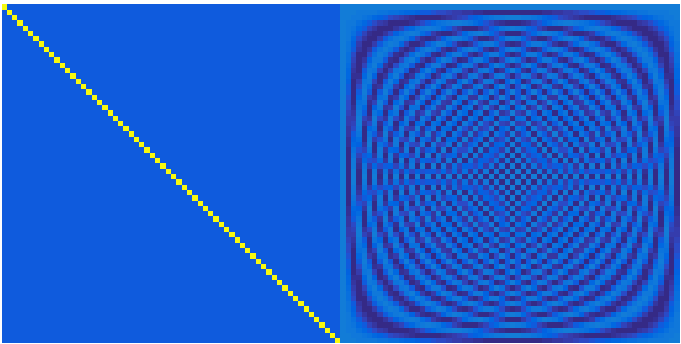
\includegraphics[width=8cm, height=3.8cm]{figures/spike_sine.pdf}};
	\end{tikzpicture}
	
	\caption{Overcomplete dictionary created by concatenation of identity (\textit{left}) and Fourier (\textit{right}) basis.}
	
	\label{fig:dictionary}
	
\end{figure}
%
Now we can create a signal which is a mixture of spikes and sinusoids. As we know that the first half of our matrix $\boldsymbol{\Psi}$ contains spike functions and the second half corresponds to sine functions, we can construct random sparsity pattern with sparsity $K$ for the vector $\boldsymbol{s}$ (of size $2N$) such that some of the non-zero entries fall into the first half and some in the second half of the vector, and then compute $\boldsymbol{x}=\boldsymbol{\Psi} \boldsymbol{s}$ to obtain a signal which is a mixture of impulses and sinusoids (see~Fig.~\ref{fig:example_signal_spectrum}a).
%
\begin{figure}
	\centering
	\begin{tikzpicture}
		\node[anchor=center, inner sep = 0](rec1) at (0,0)
		{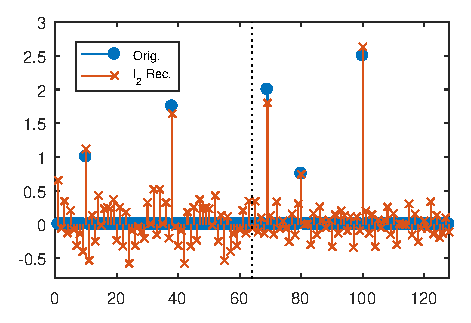
\includegraphics[width=0.84\columnwidth]{figures/example_spectrum_orig.eps}};
		
		\node[anchor=center, inner sep = 0](rec1) at (0, 8.6/1.618)
		{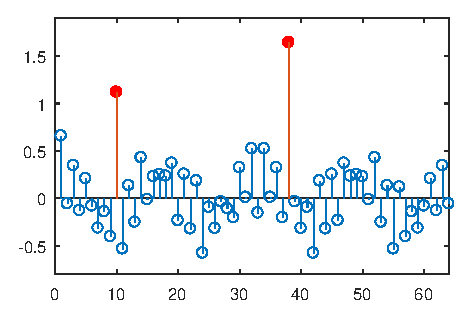
\includegraphics[width=0.84\columnwidth]{figures/example_signal.eps}};
		
		
		\filldraw[fill=white, draw=black] (3,  7.6) rectangle (3+0.4, 7.6-0.4) node[pos=0.5] {a};
		\filldraw[fill=white, draw=black] (3,  2.25) rectangle (3+0.4, 2.25-0.4) node[pos=0.5] {b};
		
	\end{tikzpicture}
	
	\caption{Example: a) arbitrary signal which consists of a mixture of two spikes (\textit{red}) and three sines of different frequency (\textit{blue}), b) spectrum of the original sparse signal (\textit{blue}) and minimum energy decomposition using $l_2$-norm. Notice that the spectrum obtained using $l_2$-norm is not sparse. The vertical dashed line separates spike (\textit{left}) and sine (\textit{right}) part of the spectrum.}
	
	\label{fig:example_signal_spectrum}
\end{figure}




%As we said before, there is an infinite number of ways to decompose signal $\boldsymbol{x}$ using atoms of our overcomplete dictionary. The most natural way would be to use certain basis functions which correspond to previously selected basis function indices and by doing so we get the sparsest possible representation. 

%Another way we can get representation for $\boldsymbol{x}$ is by applying $\boldsymbol{\Psi^*}$ and by dividing the result by 2. Since $\boldsymbol{\Psi}\boldsymbol{\Psi^*}=2\boldsymbol{I}$, we get reproducing formula for $\boldsymbol{x}$:
%%
%\begin{equation}
%\boldsymbol{x}=\frac{1}{2}\boldsymbol{\Psi}(\boldsymbol{\Psi^*}\boldsymbol{x})
%\end{equation}

We can apply $\boldsymbol{s}=\frac{1}{2}\boldsymbol{\Psi^*}\boldsymbol{x}$ and get a basis representation that corresponds to the minimum energy decomposition of our signal into a coefficient vector $\boldsymbol{s}$ that represents signal $\boldsymbol{x}$. Minimum energy decomposition corresponds to $l_2$-norm minimization. Unfortunately, minimum energy decomposition almost never yields the sparsest possible solution. The reason for this is that a vector has minimum energy when its total energy is distributed over all the coefficients of the vector. $l_2$-norm minimization gives us a solution that is dense, and has small values diffused over all coefficients (see~Fig.~\ref{fig:example_signal_spectrum}b).

In our example, we synthetically produced a signal with only $K$ coefficient representation in overcomplete basis $\boldsymbol{\Psi}$ and we want to find a decomposition that yields a signal decomposition that is $K$ sparse. Since the goal of finding the sparsest possible representation of signal $\boldsymbol{x}$ over some basis $\boldsymbol{\Psi}$ is equivalent to finding the solution with the smallest number of nonzero elements in the basis coefficient vector $\boldsymbol{s}$ we will use $l_0$-pseudo-norm to find the solution. Sparse signal recovery can be formulated as finding minimum-cardinality solution to a constrained optimization problem. 


%In the noiseless case, our constraint is simply $\boldsymbol{x}=\boldsymbol{\Psi} \boldsymbol{s}$, while in the noisy case (assuming Gaussian noise), the solution must satisfy $\Vert \boldsymbol{x}-\boldsymbol{x^*}\Vert_2\leq\epsilon$ where $\boldsymbol{x^*}=\boldsymbol{\Psi} \boldsymbol{s}$ is the hypothetical noiseless representation and the actual representation is $\epsilon$-close to it in $l_2$-norm. The objective function is the cardinality of $\boldsymbol{s}$ (number of non-zeros) which is often denoted $\Vert \boldsymbol{x}\Vert_0$ and called $l_0$-norm of $\boldsymbol{s}$ \cite{romberg}. 

%%%%%%%%%%%%%%%%%%%%%%%%%%%%%%%%%%%%%%%%%%%%%%%%%%%%%%%%%%%%%%%%%%%%%%%%%%%%%%%%%%%%%%%%%%%%%%%%%%%%%%%%%%%
\subsection{Sparse Signal Recovery}
We will use the following notation in this section to formalize the sparse signal recovery: $\boldsymbol{x}=(x_1,...,x_N)\in \mathbf{R}^N$ is an unobserved sparse signal, $\boldsymbol{y}=(y_1,...,y_M)\in \mathbf{R}^M$ is a vector of measurements (observations), and $\boldsymbol{A}=\{a_{i,j}\}\in\mathbf{R}^{M\times N}$ is a design matrix. 

The simplest problem we are going to start with is the noiseless signal recovery from a set of linear measurements, i.e., solving for $\boldsymbol{x}$ the system of linear equations:
%
\begin{equation}
	\boldsymbol{y}=\boldsymbol{A} \boldsymbol{x}
\end{equation}
%
It is usually assumed that $\boldsymbol{A}$ is a full-rank matrix, and thus for any $\boldsymbol{y}\in\mathbf{R}^M$, the above system of linear equations has a solution. Note that when the number of unknown variables, i.e., dimensionality of the signal, exceeds the number of observations ($M<N$), the above system is underdetermined, and can have infinitely many solutions. In order to recover the signal $\boldsymbol{x}$, it is necessary to further constrain, or regularize the problem. This is usually done by introducing an objective function, or regularizer $R(\boldsymbol{x})$ to an existing loss function. Regularizer encodes additional properties of the signal, with lower values corresponding to a more desirable solution. Signal recovery is then formulated as a constrained optimization problem:
%
\begin{equation}
	\min\limits_{\boldsymbol{x}\in\mathbf{R}^N} R(\boldsymbol{x})\quad s.t.\quad \boldsymbol{y}=\boldsymbol{A}\boldsymbol{x}
\end{equation}
%
Since we want to exploit underlying sparse structure of the observed signal, $R(\boldsymbol{x})$ can be defined as the number of nonzero elements, or the cardinality of $\boldsymbol{x}$, also called the $l_0$-norm. In general, $l_q$-norms for particular values of $q$, denoted $\Vert \boldsymbol{x}\Vert_q$, or more precisely, their $q$-th power $\Vert \boldsymbol{x}\Vert_q^q$, are frequently used as regularizers $R(\boldsymbol{x})$ in constrained optimization problems.

%For $q\ge 1$, the $l_q$ norm, also called just $q$-norm of a vector $\boldsymbol{x}\in\mathbf{R}^N$ is defined as:
%%
%\begin{equation}
%\Vert \boldsymbol{x}\Vert_q=(\sum\limits_{i=1}^N\vert x_i\vert^q)^\frac{1}{q}
%\end{equation}
%%
%We can now observe the relation between cardinality and $\Vert l_q\Vert$-norms. The function $\Vert \boldsymbol{x}\Vert_0$ referred to as $l_0$-pseudo-norm of $\boldsymbol{x}$ is defined as a limit of $\Vert \boldsymbol{x}\Vert_q^q$ when $q\to0$:
%%
%\begin{equation}
%\Vert \boldsymbol{x}\Vert_0=\lim\limits_{q\to 0}\Vert \boldsymbol{x}\Vert_q^q=\lim\limits_{q\to 0}\sum\limits_{i=1}^p\vert x_i\vert^q=\sum\limits_{i=1}^p\lim\limits_{q\to 0}\vert x_i\vert^q
%\end{equation}
%%
%For each $x_i$, when $q\to 0$, $\vert x_i\vert^q\to I(x_i)$, the indicator function, which is 0 at $x=0$ and 1 otherwise. Thus, $\Vert \boldsymbol{x}\Vert_0=\sum\limits_{i=1}^p I(x_i)$, which gives exactly the number of nonzero elements of vector $\boldsymbol{x}$. 

Using the cardinality function ($l_0$-norm), we can now write the problem of sparse signal recovery from noiseless linear measurements as:
%
\begin{equation}
	\min_{\boldsymbol{x}}\Vert \boldsymbol{x}\Vert_0 \quad s.t. \quad \boldsymbol{y}=\boldsymbol{A} \boldsymbol{x}
\end{equation}
%
The above optimization problem is NP-hard and no known algorithm can solve it efficiently in polynomial time. Therefore, approximations have to be introduced. Under appropriate conditions the optimal solution can be recovered efficiently by certain approximate techniques.

First approach to approximation is a heuristic-based search such as greedy search. In greedy search method, one can start with a zero vector and keep adding nonzero coefficients one by one, selecting at each step the coefficient that leads to the best improvement in the objective function. In general, such heuristic search methods are not guaranteed to find the global optimum. However, in practice, they are simple to implement, computationally efficient and under certain conditions they are even guaranteed to recover the optimal solution.

An alternative approximation technique is the relaxation approach based on replacing an intractable objective function or constraint by a tractable one. In other words, one can either solve the exact problem approximately using greedy methods, or solve an approximate problem exactly using relaxations of the original problem. In the following section, we will discuss $l_q$-norm based relaxations, and show that the $l_1$-norm occupies a unique position among them, combining convexity with sparsity. Convex problems are easier to solve than general optimization problems because of the important property that any local minima of a convex function is also a global one~\cite{Rish2015}.

%%%%%%%%%%%%%%%%%%%%%%%%%%%%%%%%%%%%%%%%%%%%%%%%%%%%%%%%%%%%%%%%%%%%%%%%%%%%%%%%%%%%%%%%%%%%%%%%%%%%%%%%%%%
\subsection{Convex Relaxations of Sparse Recovery Problem}

We will now focus on different $l_q$-norms as possible relaxations of the $l_0$-norm. These functions are convex for $q\geq 1$ and non-convex for $q<1$. For example, $l_2$-norm (Euclidean norm) would be a natural first choice as a relaxation of $l_0$-norm because of its convexity and the existence of closed form solution. However, we already showed that solution obtained using $l_2$-norm reconstruction in not sparse.
%
%Our sparse recovery problem using $l_2$-norm writes:
%%
%\begin{equation} \label{eq:l2_optimization}
%	\min\limits_{\boldsymbol{x}}\Vert \boldsymbol{x}\Vert_2^2 \quad s.t. \quad \boldsymbol{y}=\boldsymbol{A} \boldsymbol{x}
%\end{equation}
%
%Using $l_2$-norm as an objective has several advantages some of which are its convexity and thus its property that it has a unique minimum, and finally it solution is available in a closed form. The closed form solution to this problem is also known as pseudo-inverse solution of $\boldsymbol{y}=\boldsymbol{A}\boldsymbol{x}$ when $\boldsymbol{A}$ has more columns than rows (we assume that $\boldsymbol{A}$ is full-rank, i.e. all of its rows are linearly independent). However, despite its convenient properties, $l_2$-norm has a serious drawback when it comes to sparse recovery. As we already stated before, the optimal solution obtained by pseudo-inverse is practically never sparse. 
%

%To understand why the $l_2$-norm does not promote the solution sparsity while the $l_1$-norm does, and to understand the convexity and sparsity-inducing properties of $l_q$-norms in general, let us consider the geometry of a sparse recovery problem, where $\Vert \boldsymbol{x}\Vert_q^q$ replaces the original cardinality objective $\Vert \boldsymbol{x}\Vert_0$ :
%%
%\begin{equation} \label{eq:lq_optimization}
%\min\limits_{\boldsymbol{x}}\Vert \boldsymbol{x}\Vert_q^q \quad s.t. \quad \boldsymbol{y}=\boldsymbol{A} \boldsymbol{x}
%\end{equation}
%
%Sets of vectors with same value of the function $f(\boldsymbol{x})$, i.e. $f(\boldsymbol{x})=const$, are called the level sets of $f(\boldsymbol{x})$. For example, the level sets of $\Vert \boldsymbol{x}\Vert_q^q$ function are vector sets with same $l_q$-norm. A set of vectors satisfying $\Vert \boldsymbol{x}\Vert_q^q \leq r^q$ is called an $l_q$-ball of radius $r$; its “surface” (set boundary) is the corresponding level set $\Vert \boldsymbol{x}\Vert_q^q = r^q$. Note that the corresponding $l_q$-balls bounded by the level sets are convex for $q\geq 1$ (line segments between a pair of its points belong to the ball), and non-convex for $0<q<1$ (line segments between a pair of its points do not always belong to the ball).

From a geometric point of view, solving the sparse recovery problem is equivalent to “blowing up” $l_q$-balls with the center at the origin, i.e., increasing their radius, starting from 0, until they touch the hyperplane $\boldsymbol{y}=\boldsymbol{A} \boldsymbol{x}$. The resulting point is the minimum $l_q$-norm vector that is also a feasible point, i.e. it is the optimal solution of the sparse recovery problem (see~Fig.~\ref{fig:lq_balls}b).

Note that when $q\leq 1$, $l_q$-balls have sharp “corners” on the coordinate axis, corresponding to sparse vectors, since some of their coordinates are zero, but $l_q$-balls for $q>1$ do not have this property. Thus, for $q \leq 1$, $l_q$-balls are likely to meet the hyperplane $\boldsymbol{y}=\boldsymbol{A} \boldsymbol{x}$ at the corners, thus producing sparse solutions, while for $q>1$ the intersection practically never occurs at the axes, and thus solutions are not sparse (see~Fig.~\ref{fig:lq_balls}a).

Within the family of $l_q$-norms, only those with $q\geq 1$ are convex, but only those with $0<q\leq 1$ are sparsity-enforcing. The only function within that family that has both useful properties is therefore $\Vert \boldsymbol{x}\Vert_1$, i.e. the $l_1$-norm \cite{Rish2015}. This unique combination of sparsity and convexity is the reason for the widespread use of $l_1$-norms in the modern sparse signal recovery field. Optimization problem using $l_1$-norm writes:
\begin{equation} \label{eq:l1_optimization}
	\min\limits_{\boldsymbol{x}}\Vert \boldsymbol{x}\Vert_1 \quad s.t. \quad \boldsymbol{y}=\boldsymbol{A} \boldsymbol{x}
\end{equation}
%
%
\begin{figure}
	\centering
	\begin{tikzpicture}
		\node[anchor=center](rec2) at (-0.125, 0)
		{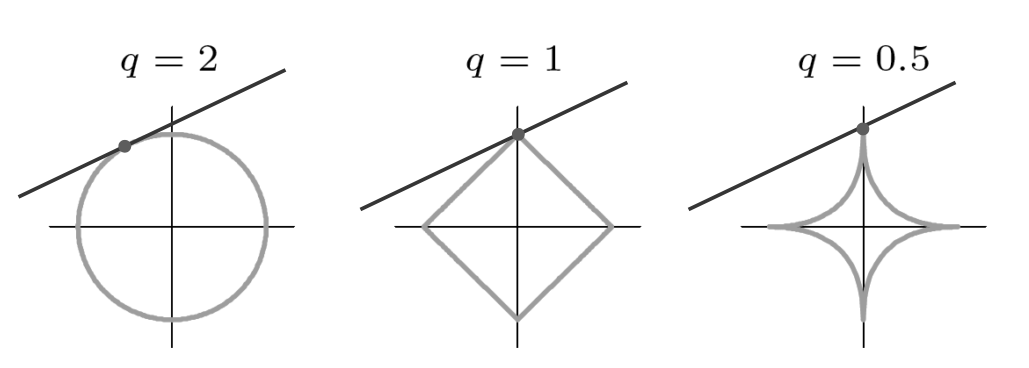
\includegraphics[width=8.6cm]{figures/lq_balls_solution.png}};
		
		\node[anchor=center](rec2) at (0, 3)
		{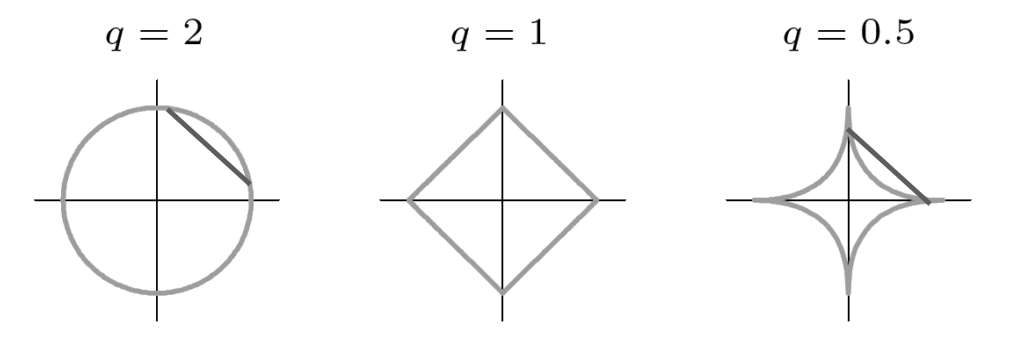
\includegraphics[width=8.6cm]{figures/lq_balls.png}};
		
		
		\filldraw[fill=white, draw=black] (-4.2,  4.5) rectangle (-4.2+0.4, 4.5-0.4) node[pos=0.5] {a};
		\filldraw[fill=white, draw=black] (-4.2,  1.2) rectangle (-4.2+0.4, 1.2-0.4) node[pos=0.5] {b};
		
	\end{tikzpicture}
	
	\caption{a) Among the family of $l_q$-norms, only $l_1$-norm has both necessary properties for successful recovery of sparse signals, i.e. it induces sparsity and is convex. b) Optimization of sparse recovery problem as inflation of the origin-centered $l_q$-balls until they meet the set of feasible points~$\boldsymbol{A}\boldsymbol{x}~=~\boldsymbol{y}$.~\cite{Rish2015}}
	\label{fig:lq_balls}
	
\end{figure}





%%%%%%%%%%%%%%%%%%%%%%%%%%%%%%%%%%%%%%%%%%%%%%%%%%%%%%%%%%%%%%%%%%%%%%%%%%%%%%%%%%%%%%%%%%%%%%%%%%%%%%%%%%%
%%%%%%%%%%%%%%%%%%%%%%%%%%%%%%%%%%%%%%%%%%%%%%%%%%%%%%%%%%%%%%%%%%%%%%%%%%%%%%%%%%%%%%%%%%%%%%%%%%%%%%%%%%%
\section{Compressive Sensing Theoretical Framework} \label{sec:3}
Compressive sensing (CS) offers a theoretical framework for simultaneous sensing and compression of finite-dimensional vectors, that relies on dimensionality reduction. In compressive sensing, the signal is not measured via standard point samples but rather through the projection by a measurement matrix $\boldsymbol{\Phi}$:
%
\begin{equation}
	\boldsymbol{y}=\boldsymbol{\Phi} \boldsymbol{x}=\boldsymbol{\Phi} \boldsymbol{\Psi} \boldsymbol{s}=\boldsymbol{A} \boldsymbol{s}
\end{equation}
%
where $\boldsymbol{\Phi}$ is an $M\times N$ measurement matrix and $\boldsymbol{y}\in\mathbf{R}^M$ is a set of $M$ measurements or samples where $M$ can be much smaller than the original dimensionality of the signal, hence the name compressive sensing. We introduce $\boldsymbol{A}=\boldsymbol{\Phi}\boldsymbol{\Psi}$ and refer to it as the design matrix for compressive sensing (\ref{fig:cs_matrices}). The central problem of compressive sensing is reconstruction of high-dimensional sparse signal representation $\boldsymbol{x}$ from a low-dimensional linear observation $\boldsymbol{y}$, also called the measurement vector. 
%
\begin{figure}
	\begin{tikzpicture}
		\node[anchor=center, inner sep = 0](rec1) at (0,0)
		{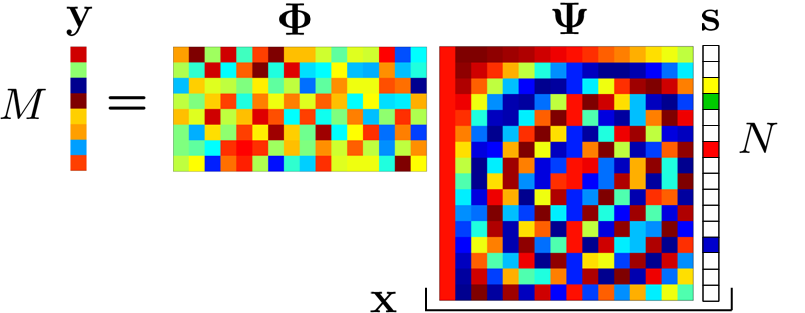
\includegraphics[width=8.6cm]{figures/cs_matrices.png}};
	\end{tikzpicture}
	

	\caption{Matrix form representation of compressive sensing problem. Measurement vector is obtained through projection of an unknown signal $\boldsymbol{s}$ that is sparse in some basis $\boldsymbol{\Psi}$ by a measurement matrix $\boldsymbol{\Phi}$. \cite{cs_matrices_url}}
	
	\label{fig:cs_matrices}
\end{figure}



Ideally, the measurement matrix $\boldsymbol{\Phi}$ is designed to reduce the number of measurements $M$ as much as possible while allowing for recovery of a wide class of signals and providing non-adaptive sampling scheme. However, the fact that $M<N$ renders the matrix rank-deficient, meaning that it has a nonempty null-space, which in turn implies that for any particular signal $\boldsymbol{x}_0\in \mathbf{R}$, an infinite number of signals will yield the same measurements $\boldsymbol{y}_0=\boldsymbol{\Phi} \boldsymbol{x}_0 = \boldsymbol{\Phi} \boldsymbol{x}$ for chosen measurement matrix $\boldsymbol{\Phi}$. The motivation behind the design of the matrix $\boldsymbol{\Phi}$ is to allow for distinct signals ($\boldsymbol{x},\,\boldsymbol{x'}$) within a class of signals of interest to be uniquely identifiable using sparse optimization techniques from their measurements ($\boldsymbol{y},\,\boldsymbol{y'}$), even though $M\ll N$~\cite{Duarte2011}.

%%%%%%%%%%%%%%%%%%%%%%%%%%%%%%%%%%%%%%%%%%%%%%%%%%%%%%%%%%%%%%%%%%%%%%%%%%%%%%%%%%%%%%%%%%%%%%%%%%%%%%%%%%%
\subsection{Uniqueness of Compressive Sensing Recovery Problem}
In this section we will discuss when the solutions of the $l_0$- and $l_1$- norm minimization problems are unique. The main design criteria for matrix $\boldsymbol{A}$ is to enable the unique identification of a signal of interest $\boldsymbol{x}$ from its measurements $\boldsymbol{y}=\boldsymbol{A}\boldsymbol{x}$. Clearly, when we consider the class of $K$-sparse signals $\Sigma_K$, the number of measurements has to be $M>K$ for any matrix design, since the identification problem has $K$ unknowns.

We will now determine properties of $\boldsymbol{A}$ that guarantee that distinct signals $\boldsymbol{x},\,\boldsymbol{x'}\in \Sigma_K,\, \boldsymbol{x}\neq \boldsymbol{x'}$, lead to different measurement vectors $\boldsymbol{A}\boldsymbol{x}\neq \boldsymbol{A}\boldsymbol{x'}$. In other words, we want each vector $\boldsymbol{y}\in \mathbf{R}^M$ to be matched to at most one vector $\boldsymbol{x}\in \Sigma_K$ such that $\boldsymbol{y}=\boldsymbol{A}\boldsymbol{x}$.

%%%%%%%%%%%%%%%%%%%%%%%%%%%%%%%%%%%%%%%%%%%%%%%%%%%%%%%%%%%%%%%%%%%%%%%%%%%%%%%%%%%%%%%%%%%%%%%%%%%%%%%%%%%
\subsection{Sensing Matrix Properties}
\subsubsection{Spark}
A key relevant property of the matrix in this context is its spark \cite{donoho2003optimally}. Given an $M\times N$ matrix $\boldsymbol{A}$, its spark $spark(\boldsymbol{A})$, is defined as the minimal number of linearly dependent columns. Spark is closely related to the Kruskal's rank $krank(\boldsymbol{A})$ defined as the maximal number $k$ such that every subset of $k$ columns of the matrix $\boldsymbol{A}$ is linearly independent~\cite{kruskal1977three}. We can now write the relation between \textit{spark} and \textit{krank} as:
%
\begin{equation} \label{eq:skrank}
	spark(\boldsymbol{A})=krank(\boldsymbol{A})+1\quad \text{and} \quad rank(\boldsymbol{A})\geq krank(\boldsymbol{A})
\end{equation}

By definition, the vectors in the null-space of the matrix $\boldsymbol{A}\boldsymbol{x}=\boldsymbol{0}$ must satisfy $\Vert \boldsymbol{x}\Vert_0\geq spark(\boldsymbol{A})$, since these vectors linearly combine columns from $\boldsymbol{A}$ to give the zero vector, and at least \textit{spark} such columns are necessary by definition. Sparse recovery solution uniqueness via spark can be stated as: if $spark(\boldsymbol{A})>2K$, then for each measurement vector $\boldsymbol{y}\in\mathbf{R}^M$ there exists at most one signal $\boldsymbol{x}\in\Sigma_K$ such that $\boldsymbol{y}=\boldsymbol{A}\boldsymbol{x}$ \cite{Rish2015}. The singleton bound yields that the highest spark of an matrix $\boldsymbol{A}\in\mathbf{R}^{M\times N}$ with $M<N$ is less than or equal to $M+1$ and using the before stated theorems we get the requirement $M\geq 2K$.

While \textit{spark} is useful notion for proving the exact recovery of a sparse optimization problem, it is NP-hard to compute since one must verify that all sets of columns of a certain size are linearly independent. Thus, it is preferable to use properties of $\boldsymbol{A}$ which are easily computable to provide recovery guarantees.

\subsubsection{Coherence}
The coherence $\mu(\boldsymbol{A})$ of a matrix is the largest absolute inner product between any two columns of matrix $\boldsymbol{A}$:
%
\begin{equation} \label{eq:coherence}
	\mu(\boldsymbol{A})=\max\limits_{1\leq i\neq j\leq N}\frac{\langle a_i,
		a_j\rangle}{\Vert a_i\Vert_2 \Vert a_j\Vert_2}
\end{equation}
%
For any matrix $\boldsymbol{A}$,
\begin{equation} \label{eq:coherence_spark}
	spark(\boldsymbol{A})\geq 1+\frac{1}{\mu(\boldsymbol{A})}
\end{equation}
%
%Quite simple way to read the coherence is from the absolute value Gram matrix \cite{Elad2010}. Gram matrix is defined as $\boldsymbol{G}=\boldsymbol{A'}\boldsymbol{A}$ where we are considering conjugate transpose of the matrix $\boldsymbol{A}$. To read the coherence from Gram matrix, we reject the diagonal elements since they correspond to the inner product of an atom with itself (for a properly normalized dictionary they should be 1 anyway). Since $\boldsymbol{G}$ is symmetric we need to look only upper triangular half of it to read off the coherence. The value of coherence $\mu(\boldsymbol{A})$ is equal to largest value in upper triangular part of matrix $\boldsymbol{A}$ with diagonal excluded. 
%
It can be shown that $\mu(\boldsymbol{A})\in \big[\sqrt{\frac{N-M}{M(N-1)}}, 1\big]$. The lower bound is known as the Welch bound. Note that when $N>>M$, the lower bound is approximately $\mu(\boldsymbol{A})\geq \frac{1}{\sqrt{M}}$~\cite{donoho2003optimally}. In our example with overcomplete dictionary with spikes and sines basis, the coherence exactly corresponds to the Welch bound. That confirms our statement that spikes and sines are mutually completely incoherent. In~\cite{Pereira2014}, a method to design sensing matrices with minimum coherence to a given sparsifying orthogonal basis was proposed. They provided a mathematical proof of the optimality in terms of coherence minimization for the proposed sensing matrices.

\subsubsection{Restricted Isometry Property}
The prior properties of the CS design matrix provide guarantees of uniqueness when the measurement vector $\boldsymbol{y}$ is obtained without error. There can be two sources of error in the measurements: inaccuracies due to noise at sensing stage (in the form of additive noise $\boldsymbol{y}=\boldsymbol{A}\boldsymbol{x}+noise$) and inaccuracies due to mismatches between the design matrix used during recovery and that implemented during acquisition (in the form of multiplicative noise $\boldsymbol{A'}=\boldsymbol{A}+\boldsymbol{A}_{noise}$). Under these sources of error, it is no longer possible to guarantee uniqueness, but it is desirable for the measurement process to be tolerant to both types of error. To be more formal, we would like the distance between the measurement vectors for two sparse signals $\boldsymbol{y}=\boldsymbol{A}\boldsymbol{x}$ and $\boldsymbol{y'}=\boldsymbol{A}\boldsymbol{x'}$ to be proportional to the distance between the original signal vectors $\boldsymbol{x}$ and $\boldsymbol{x'}$. Such a property allows us to guarantee that for small enough noise, two sparse vectors that are far apart from each other cannot lead to the same noisy measurement vector. This behavior has been formalized into the restricted isometry property (\textit{RIP}) \cite{Moreira2014, Romberg2013, CANDES2008589, Blanchard2011}. 

A matrix $M\times N$ $\boldsymbol{A}$ is said to satisfy the $(K,\delta)$-restricted isometry property ($(K,\delta)$-RIP) if, for all $\boldsymbol{x}\in\Sigma_K$:

\begin{equation} \label{eq:rip}
	(1-\delta)\Vert \boldsymbol{x}\Vert^2_2\leq\Vert\boldsymbol{\Phi }\boldsymbol{x}\Vert_2^2\leq(1+\delta)\Vert\boldsymbol{x}\Vert_2^2
\end{equation}
%
where $\Sigma_K$ represents the set of all length-$N$ vectors with $K$ non-zero coefficients and $\delta \in (0,1)$. In words, the $(K,\delta)$-RIP ensures that all sub-matrices of $\boldsymbol{A}$ of size $M\times K$ are close to an isometry, and therefore are distance-preserving. This property suffices to prove that the recovery is stable to presence of additive noise and the RIP also leads to stability with respect to the multiplicative noise.

The definition of the RIP is closely related to the frame theory and Riesz bases which were developed in \cite{duffin1952class} to provide theoretical framework for band-limited signal reconstruction from irregularly spaced samples. RIP is consistent with the thought of spreading energy behind random sensing matrices so measurement $\boldsymbol{y}$ does not shrink or expand too much comparing to the original signal $\boldsymbol{x}$. RIP can be viewed as a modified frame theory:
%
\begin{equation} \label{eq:frame}
	A\Vert \boldsymbol{x}\Vert^2\leq\Vert\boldsymbol{\Phi }\boldsymbol{x}\Vert^2\leq B\Vert\boldsymbol{x}\Vert^2
\end{equation}
%
where the frame bounds are $0<A\leq B \leq 2$.

In~\cite{Candes2011}, authors provided a simple compressive sensing framework which applies all the standard compressive sensing models with addition of some new ones. They established a probabilistic and RIP-less CS theory that states that the RIP property is not necessarily needed to accurately recover nearly sparse vectors from noisy compressive measurements. This represents a significant advance with application to many real world situations where RIP may be hard to check or even might not hold.

\subsection{Asymptotic Structure in Compressive Sensing}
CS theory presented in the previous sections presents traditional view on the compressive sensing. In recent years, novel compressive sensing theory was introduced by Roman, Adcock and Hansen in \cite{Adcock2013, Adcock2015, Roman2014, Adcock}. They introduce new pillars of compressive sensing, namely \textit{asymptotic incoherence}, \textit{asymptotic sparsity} and \textit{multilevel sampling} which replace the traditional notion of sparsity (there are $K$ important coefficients in the vector to be recovered and their location is arbitrary), incoherence (values in the measurement matrix should be dense and uniformly spread out) and uniform random subsampling. Traditional compressive sensing states that the signal sampling strategy is completely independent of the location of the nonzero coefficients. In their flip test, Adcock et al. show that sparsity alone does not dictate the compressive sensing reconstruction quality and that the optimal sampling strategy must indeed depend on the signal structure.

Assume that $\boldsymbol{x}$ is an image vector, $\boldsymbol{\Phi}$ is some measurement matrix and $\boldsymbol{\Psi}$ is a transformation basis matrix. We can define new matrix $\boldsymbol{A}=\boldsymbol{R}_\Omega \boldsymbol{\Phi}\boldsymbol{\Psi}$, where $\boldsymbol{R_\Omega}$ is reduction matrix corresponding to some subsampling pattern $\Omega \subseteq \{1,...,N\}$ with $\vert \Omega\vert = M$, and our measurement vector as $\boldsymbol{y}=\boldsymbol{R}_\Omega\boldsymbol{\Phi}\boldsymbol{\Psi}\boldsymbol{s}=\boldsymbol{A}\boldsymbol{s}$. We can now solve standard sparse optimization problem in the form of Eq. \ref{eq:l1_optimization} and obtain sparse representation $\boldsymbol{s}$ of the image. If the sparsity is the right model as traditional CS theory states, we should be able to flip the reconstructed coefficients to obtain $\boldsymbol{s}_f$ since $\Vert\boldsymbol{s}\Vert_0=\Vert\boldsymbol{s}_f\Vert_0$. Next, we can define new measurement vector using the flipped coefficients $\boldsymbol{{y'}}=\boldsymbol{A}\boldsymbol{s}_f$ and again solve the sparse optimization problem using the new measurement vector $\boldsymbol{{y'}}$ and get the estimation of the sparse vector $\boldsymbol{s}_{f}'$ which we flip again to get $\boldsymbol{{s'}}$. The image estimation $\boldsymbol{{x'}}$ is then calculated as $\boldsymbol{{x}'}=\boldsymbol{\Psi}\boldsymbol{{s'}}$. If sparsity is the right model, estimation using the direct coefficient recovery should be equal to flipped coefficients recovery $\boldsymbol{{x}=\boldsymbol{x'}}$ which is not the case, as shown in Fig.~\ref{fig:flip_test_reconstruction}. 

%\begin{equation}
%	\min_{\boldsymbol{s}} \Vert s\Vert_1 \quad s.t. \quad \boldsymbol{A}\boldsymbol{s}=\boldsymbol{y} 
%\end{equation}
%
\begin{figure}
	\centering
	\begin{tikzpicture}
	\node[anchor=center, inner sep = 0](rec1) at (0,0)
	{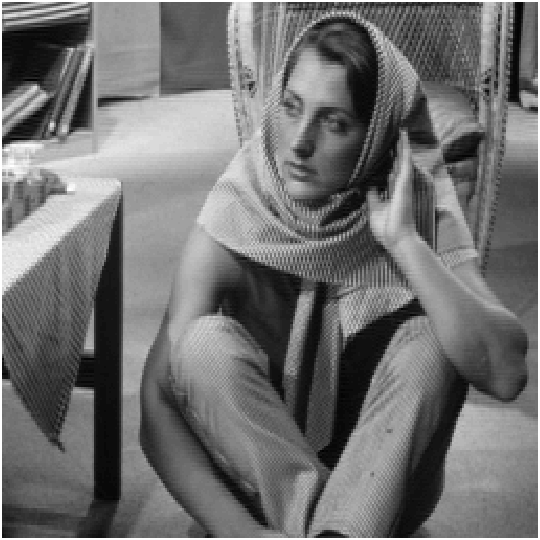
\includegraphics[width=4.3cm, height=4cm]{figures/flip_test_reconstruction_normal.pdf}};
	
	\node[anchor=center, inner sep = 0](rec1) at (4.5,0)
	{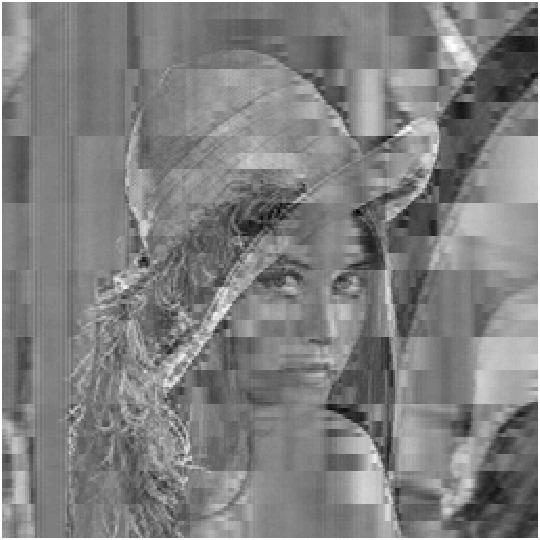
\includegraphics[width=4.3cm, height=4cm]{figures/flip_test_reconstruction_flip.pdf}};
	\end{tikzpicture}
	
	
	\caption{Flip test performed on \textit{Barb} image. Left image shows recovery from direct wavelet coefficients while right image shows reconstruction using flipped coefficients. Measurement matrix used in the flip test is Walsh-Hadamard matrix, and the transformation basis is Haar's wavelet. Flipped coefficients recovery is substantially worse than the direct coefficient recovery.}
	
	\label{fig:flip_test_reconstruction}
\end{figure}

%%%%%%%%%%%%%%%%%%%%%%%%%%%%%%%%%%%%%%%%%%%%%%%%%%%%%%%%%%%%%%%%%%%%%%%%%%%%%%%%%%%%%%%%%%%%%%%%%%%%%%%%%%%
\subsection{Structure in Measurement Matrix}
In the previous sections, we assumed use of randomized compressive sensing matrices whose entries are obtained independently from a standard probability distribution. While the proposed matrix choice satisfies the conditions imposed on the CS measurement matrix, it has numerous disadvantages when it comes to real-world applications. One disadvantage is the cost of multiplying arbitrary matrices with high-dimensional signals. Furthermore, often the physics of the sensing modality and the capabilities of the measurement device limit the freedom in choosing measurement matrices. 

To overcome these problems, structured measurement matrices were proposed and \cite{Li2015} provides an extensive overview. There are numerous ways of introducing structure into the measurement matrix design. One idea is to simply select a basis that is incoherent to the sparsity basis $\boldsymbol{\Psi}$, and obtain CS measurements by selecting a subset of the coefficients of the signal in the chosen basis \cite{Candes2007}. Use of subsampled circulant matrices as CS measurement matrices was inspired by applications in channel estimation and multiuser detection \cite{bajwa2007toeplitz, haupt2010toeplitz, yinpractical}. Furthermore, separable matrices provide computationally efficient alternatives to measure high-dimensional data. These matrices use Kronecker product \cite{schacke2013kronecker} to create sparsity basis which simultaneously exploits the sparsity properties of a multidimensional signal along each of its dimensions \cite{Rivenson2009, Duarte2012}.  

%%%%%%%%%%%%%%%%%%%%%%%%%%%%%%%%%%%%%%%%%%%%%%%%%%%%%%%%%%%%%%%%%%%%%%%%%%%%%%%%%%%%%%%%%%%%%%%%%%%%%%%%%%%
%%%%%%%%%%%%%%%%%%%%%%%%%%%%%%%%%%%%%%%%%%%%%%%%%%%%%%%%%%%%%%%%%%%%%%%%%%%%%%%%%%%%%%%%%%%%%%%%%%%%%%%%%%%
\section{Overcomplete Dictionaries and Dictionary Learning} \label{sec:4}

Sparsifying basis that leads to sparse representations of signals can either be chosen as a pre-specified set of basis functions, or designed by adapting the functions to fit a given set of signal examples. We refer to the first approach as analytic approach in which a mathematical model of the data is formulated, and an analytic construction is developed to efficiently represent the model. This procedure leads to implicit dictionaries which have efficient implementations, but lack adaptability. Some examples of implicit dictionaries are: Fourier basis, wavelets \cite{daubechies1992ten}, curvelets \cite{starck2002curvelet}, contourlets \cite{do2002contourlets}, shearlets \cite{guo2007optimally} and bandelets \cite{le2005sparse}. 

The second approach suggests using machine learning techniques to infer the dictionary from a set of examples~\cite{olshausen1996emergence, Petrov2012, Rubinstein, Christen2010}. In this case, the dictionary is typically represented as an explicit matrix, and a training algorithm is employed to adapt the matrix coefficients to the examples and the final goal is to find the dictionary $\boldsymbol{D}$ that yields the sparsest representation of the training signals. 

The ultimate sparse-coding objective is to find both $\boldsymbol{D}$ and $\boldsymbol{X}$ that yield the sparsest representation of the data $\boldsymbol{Y}$, subject to some acceptable approximation error $\epsilon$:

\begin{equation} \label{eq:dictionary_learning}
	\min\limits_{\boldsymbol{D}, \boldsymbol{X}}\sum\limits_{i=1}^N \Vert \boldsymbol{x}_i\Vert_1 \quad s.t.\quad \Vert \boldsymbol{Y}-\boldsymbol{D}\boldsymbol{X}\Vert_2\leq \epsilon
\end{equation}

Note that this problem formulation looks very similar to the classical sparse signal recovery problem, only with two modifications: dictionary $\boldsymbol{D}$ is now included as an unknown variable that we must optimize over, and there are multiple observed samples and the corresponding sparse signals rather than just one. 
%
\begin{figure}[h]
	
	\begin{tikzpicture}
	\node[anchor=center, inner sep = 0](rec1) at (0,0)
	{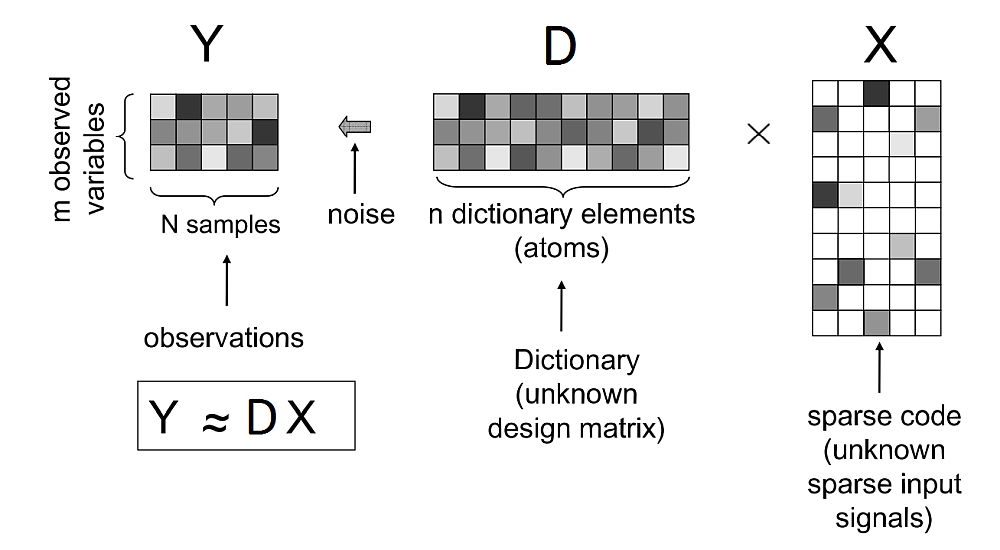
\includegraphics[width=9cm]{figures/dictionary_learning.png}};
	
	\end{tikzpicture}
		
	\caption{Dictionary learning matrix form representation \cite{Rish2015}.}
	
	\label{fig:dictionary_learning}
	
\end{figure}
Several different dictionary learning algorithms have been introduced over the past years: method of optimal directions (MOD) \cite{engan1999method}, K-SVD \cite{Aharon2006} and online-dictionary learning \cite{mairal2010online} are the most popular ones. First two methods are batch methods which attempt to learn a dictionary directly from the full data set which makes them computationally inefficient. Third method belongs to a family of online dictionary learning methods where learning is done incrementally, one training sample (or a batch of samples) at a time, which makes them scale better in applications where a very large number of training examples exists.
%
\begin{figure}[tbp]
	\centering
	\begin{tikzpicture}
	\node[anchor=center, inner sep = 0](rec1) at (0,0)
	{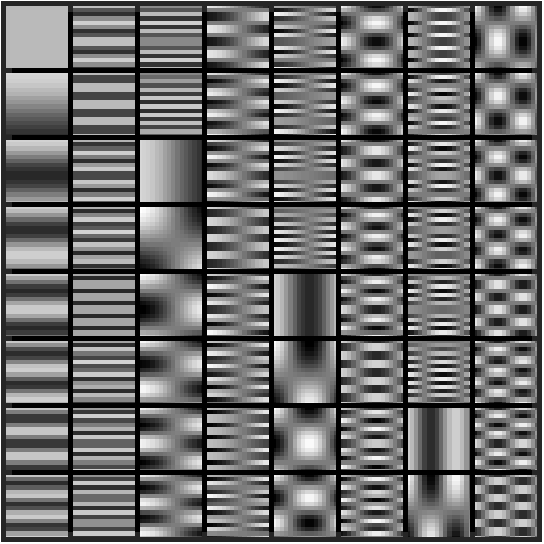
\includegraphics[width=4.3cm, height=4cm]{figures/dct_dict.pdf}};
	
	\node[anchor=center, inner sep = 0](rec1) at (4.5,0)
	{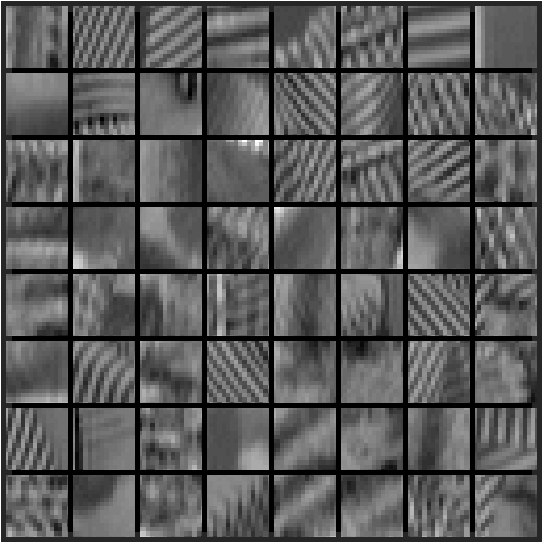
\includegraphics[width=4.3cm, height=4cm]{figures/learned_dict.pdf}};
	\end{tikzpicture}
	
	
	\caption{Dictionary learning performed on \textit{Barb} image. Left image shows part of initial overcomplete DCT dictionary and right image shows part of the learned dictionary using online dictionary learning algorithm. Notice that the high-frequency content that is image specific is captured in the learned dictionary.}
	
	\label{fig:flip_test_reconstruction}
\end{figure}



In \cite{Rubinstein2010}, an efficient and flexible dictionary structure is proposed which bridges the gap between implicit dictionaries, which have efficient implementations yet lack adaptability, and explicit dictionaries, which are fully adaptable but costly in terms of computational resources. The proposed sparse dictionary is based on a sparsity model of the dictionary atoms over a base dictionary, and takes the form $\boldsymbol{D}=\boldsymbol{\Psi}\boldsymbol{A}$ where $\boldsymbol{\Psi}$ is a fixed base dictionary and $\boldsymbol{A}$ is sparse. The sparse dictionary model suggests that each atom of the dictionary has itself a sparse representation over some prespecified base dictionary $\boldsymbol{\Psi}$ (see Fig.~\ref{fig:double_sparsity}).

\begin{figure}
	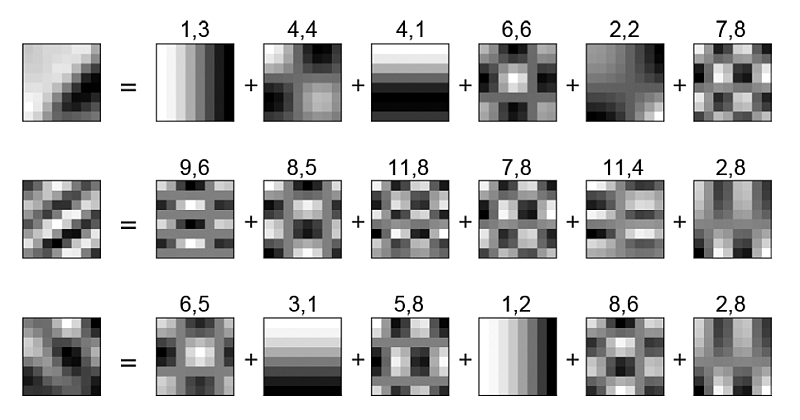
\includegraphics[width=8.6cm]{figures/double_sparsity}
	
	\caption{Some atoms of sparse dictionary trained over an overcomplete DCT dictionary using Sparse K-SVD algorithm. Dictionary atoms are represented using 6 coefficients each \cite{Rubinstein2010}.}
	
	\label{fig:double_sparsity}
\end{figure}

%%%%%%%%%%%%%%%%%%%%%%%%%%%%%%%%%%%%%%%%%%%%%%%%%%%%%%%%%%%%%%%%%%%%%%%%%%%%%%%%%%%%%%%%%%%%%%%%%%%%%%%%%%%
%%%%%%%%%%%%%%%%%%%%%%%%%%%%%%%%%%%%%%%%%%%%%%%%%%%%%%%%%%%%%%%%%%%%%%%%%%%%%%%%%%%%%%%%%%%%%%%%%%%%%%%%%%%
\section{Overview of Algorithms for Sparse Recovery} \label{sec:5}

In this section we will provide a brief overview of algorithms for sparse recovery. We can write the sparse recovery problem in the case of noise as a convex $l_1$-norm relaxation of the standard $l_0$-norm minimization:
%
\begin{equation} \label{eq:l0_minimization_noisy}
	\min_{\boldsymbol{x}}\Vert\boldsymbol{x}\Vert_1 \quad s.t. \quad \Vert \boldsymbol{y}-\boldsymbol{A}\boldsymbol{x}\Vert_2\leq \epsilon
\end{equation}
Furthermore, $l_1$-norm minimization can be written in alternative unconstrained form as:
%
\begin{equation} \label{eq:lasso_unconstrained}
	\min_{\boldsymbol{x}}\frac{1}{2}\Vert \boldsymbol{y}-\boldsymbol{A}\boldsymbol{x}\Vert_2^2+\lambda\Vert\boldsymbol{x}\Vert_1
\end{equation}
%
or, for an appropriate parameter $t(\epsilon)$, denoted as $t$, the same problem can be rewritten as:
\begin{equation} \label{eq:lasso_constrained}
	\min_{\boldsymbol{x}} \Vert \boldsymbol{y}-\boldsymbol{A}\boldsymbol{x}\Vert_2^2 \quad s.t. \quad \Vert x\Vert_1 \leq t
\end{equation}
%
The above $l_1$ regularized problem in the latter two forms is known as the \textit{LASSO} (Least Absolute Shrinkage and Selection Operator) \cite{tibshirani1996regression}.

A comprehensive overview of sparse recovery algorithms is given in \cite{Zhang2015}. They categorize sparse optimization algorithms into four groups: greedy strategy approximation, constrained optimization, proximity algorithm-based optimization and homotopy algorithm-based sparse optimization. 

In the greedy strategy approximation for solving sparse representation problem, the target task is mainly to solve the sparse representation method with $l_0$-norm minimization. Because of the fact that this problem is an NP-hard problem , the greedy strategy provides an approximate solution to alleviate this difficulty. The greedy strategy searches for the best local optimal solution in each iteration with the goal of achieving the optimal holistic solution. Some of the most commonly-used greedy methods are: matching pursuit \cite{chen2001atomic}, orthogonal matching pursuit (OMP) \cite{pati1993orthogonal}, stage-wise OMP (StOMP) \cite{donoho2012sparse}, compressive sampling matching pursuit (CoSaMP) \cite{needell2009cosamp} and several others. 

As mentioned before, in the constrained optimization strategy, the core idea is to explore a suitable way to transform a non-differentiable optimization problem into a differentiable optimization problem by replacing the $l_1$-norm minimization term, which is convex but non-smooth, with a differentiable optimization term, which is convex and smooth. Some of constrained optimization strategy based algorithms are: gradient projection sparse reconstruction (GPSR) \cite{figueiredo2007gradient}, least angle regression for \textit{LASSO} (LARS) \cite{efron2004least}, truncated Newton based interior-point method (TNIPM) \cite{portugal2000truncated}, alternating direction method (ADM) \cite{yang2011alternating} and others.

In the proximity algorithm-based optimization strategy for sparse representation, the main task is to reformulate the original problem into the specific model of the corresponding proximal operator such as the soft thresholding operator, hard thresholding operator, and resolvent operator, and then exploits the proximity algorithms to address the original sparse optimization problem. Iterative shrinkage thresholding algorithm (ISTA) \cite{figueiredo2005bound}, fast iterative shrinkage thresholding algorithm (FISTA) \cite{beck2009fast}, sparse reconstruction by separable approximation (SpaRSA) \cite{Wright2009} and generalized Nesterov's algorithm (NESTA) \cite{becker2011nesta} are examples of proximity algorithm-based optimization methods.

The main idea of homotopy algorithm-based sparse representation is to solve the original optimization problems by tracing a continuous optimization problems by tracing a continuous parameterized path of solutions along with varying parameters. In contrast to LARS and OMP, the homotopy method is more favorable for sequentially updating the sparse solution by adding or removing elements from the active set. Some of the most representative homotopy based reconstruction methods are \textit{LASSO} homotopy and basis pursuit denoising (BPDN) \cite{Zhang2015}.

In \cite{qi2011using}, authors adapt the kernel trick usually used in machine learning applications to easily adapt linear algorithms to nonlinear situations. They show how the kernel trick can be used to adapt the traditional paradigm of reconstructing a linearly sparse signal from a linear set of measurements to the case of reconstructing a nonlinearly sparse signal from either nonlinear or linear measurements. The key idea is that a signal that is nonlinearly sparse can, with a proper choice of kernel, become linearly sparse in feature space. Then, reconstruction can be performed on random measurements in feature space, which can be obtained from the usual random measurements for some kernels.
%
\begin{figure*}[htbp]
	\centering
	\begin{tikzpicture}
	\node[anchor=center, inner sep = 0](rec1) at (0,0)
	{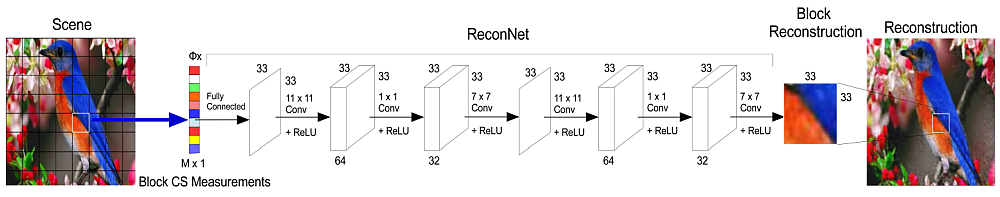
\includegraphics[width=18cm]{figures/reconnet.png}};
	
	\end{tikzpicture}
	
	\caption{Overview of deep neural network design for non-iterative block CS image recovery algorithm. The scene is divided into non-overlapping blocks. Each block is reconstructed by feeding in the corresponding CS measurements to the deep network. The reconstructed blocks are then arranged appropriately to form the image reconstruction. The input to the network is an $M$-dimensional vector of compressive measurements, denoted by $\boldsymbol{\Phi}\boldsymbol{x}$, where $\boldsymbol{\Phi}$ is the measurement operator of size $M \times M$ where $M$ is the number of measurements and $\boldsymbol{x}$ is the vectorized image block \cite{Kulkarni2016}.}
	
	\label{fig:reconnet}
\end{figure*}

Recently, machine learning methods for learning data representations started to gain more interest in the area of compressive sensing. A non-iterative and extremely fast algorithms based on deep neural networks have recently been proposed in~\cite{Kulkarni2016, Mousavi2017, Mousavi2015}. These papers adapt different designs of deep neural network for application in compressive sensing reconstruction of images. In \cite{Kulkarni2016}, authors propose a novel convolutional neural network (CNN) architecture inspired by the work of Dong et al. \cite{Dong2016} which takes CS measurements of an image as input and outputs an intermediate image reconstruction. They showed that the images reconstructed using convolutional network outperform state-of-the-art iterative CS reconstruction algorithms under certain conditions. The convolutional neural network design is shown in Fig. \ref{fig:reconnet}. Signal recovery framework proposed in \cite{Mousavi2017} learns the inverse transformation from measurement vectors $\boldsymbol{y}$ to signals $\boldsymbol{x}$ using a special deep network architecture. When trained on a set of representative images, the network learns both a representation for the signals $\boldsymbol{x}$ and an inverse map approximating a greedy or convex recovery algorithm.

%%%%%%%%%%%%%%%%%%%%%%%%%%%%%%%%%%%%%%%%%%%%%%%%%%%%%%%%%%%%%%%%%%%%%%%%%%%%%%%%%%%%%%%%%%%%%%%%%%%%%%%%%%%
%%%%%%%%%%%%%%%%%%%%%%%%%%%%%%%%%%%%%%%%%%%%%%%%%%%%%%%%%%%%%%%%%%%%%%%%%%%%%%%%%%%%%%%%%%%%%%%%%%%%%%%%%%%
\section{Applications of Sparse Representations and Compressive Sensing} \label{sec:6}

The impact that compressive sensing and sparse signal representations had on the signal processing community is immense. There are numerous applications trying to apply the theoretical CS framework to real world problems. Still, there is a gap between the theoretical knowledge and practical implementations. In this section, we will provide an overview of existing practical applications of sparse representations and compressive sensing.

Signal compression has been a topic of interest for many years thanks to the fact that most of the natural signals are compressible in some transformation basis, thus, sparse modeling seems to be a very natural approach to signal compression. Conventional transform coding methods use predefined basis dictionaries to obtain concise representations. While predefined dictionaries are computationally efficient, they are typically limited in the ability to sparsify the observed signals. On the other hand, the proposed dictionary learning methods enable discovery of underlying structure in signals of interest and tend to provide us with sparser representations than conventional methods. In~\cite{nejati2016boosted, horev2012adaptive, skretting2011image} different overcomplete dictionaries are learned and applied to image compression problems and outperform conventional methods. Other applications of dictionary learning include image denoising \cite{Elad2008}, image inpainting \cite{Shen2009, Mairal2008} and image super-resolution \cite{yang2010image, kim2010single, yang2008image}.

The previously mentioned applications use dictionary learning for purely reconstructive tasks and we call such learning methods unsupervised learning. The final goal of reconstructive dictionary learning is to minimize the residual of reconstructing the original signals. Sparse signal representations have another natural property of being discriminative in such a way that the obtained signal representation is sparsest possible. This lead to development of different classification methods based on dictionary learning where classification is based on the corresponding reconstruction error \cite{Zhang2010, ZhuolinJiang2013} with applications on face recognition \cite{Wright2009_src} (see Fig. \ref{fig:face_recognition}) and other classification problems.
%
\begin{figure}[h]
	\centering
	\begin{tikzpicture}
		\node[anchor=center](rec1) at (0,0)
		{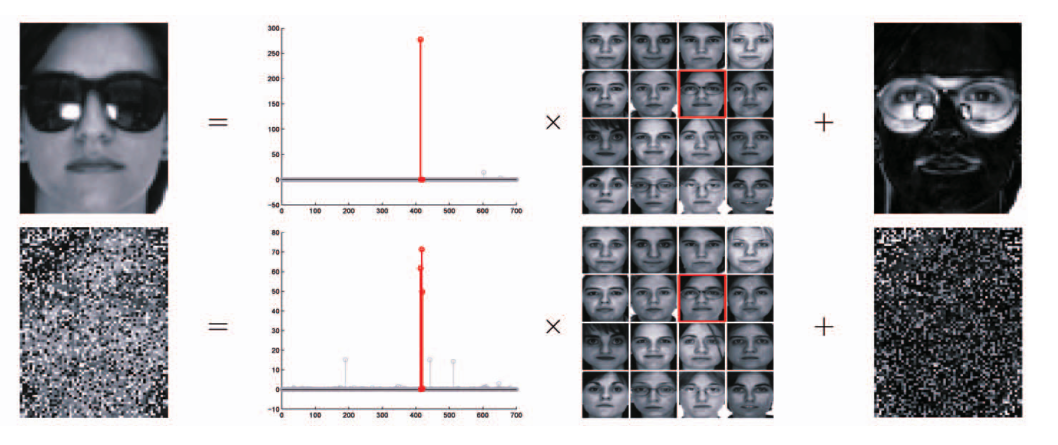
\includegraphics[width=8.8cm]{figures/face_recognition.png}};
	\end{tikzpicture}
		
	\caption{Robust face recognition using sparse coding reconstruction error. Proposed method represents a test image as a sparse linear combination of all the training images and classifies test image based on the obtained reconstruction error. \cite{Wright2009_src}}
	
	\label{fig:face_recognition}
\end{figure}

As already mentioned in the introduction, compressive sensing found its first application in MRI medical imaging because of the existing natural connection. MRI obeys two key requirements for successful application of CS: medical images are naturally compressible by sparse coding in appropriate transform domain and MRI scanners acquire encoded samples, rather than direct pixel samples. Compressive sensing improved acquisition speed and spatial resolution of MRI scans and novel applications like rapid 3D angiography, whole-heart coronary imaging and brain imaging emerged. In \cite{Geethanath2013}, Geethanath et al. give a detailed overview of applications of CS to MRI.

In compressive imaging the central idea is to design encoded, subsampled linear measurements which allow for accurate optimization-based decoding which assumes sparsity in some transform domain. Applications of compressive imaging include fluorescence microscopy, infrared microscopy, single-pixel imaging, light-field reconstructions and several others. Different designs for imaging devices based on compressive sensing have been proposed and each design tackles certain limitation of traditional imaging systems. For example, in~\cite{Reddy2011}, authors propose P2C2 (Programmable Pixel Compressive Camera) camera which consists of a normal 25fps, low resolution video camera in combination with a high resolution, high frame-rate modulating device (DMD or LCoS). This design offers inexpensive and efficient acquisition and recovery of high-resolution, high-speed frames from the captured low-res frames by exploiting temporal redundancy in the form of brightness constancy and spatial redundancy through transform domain sparsity in a convex optimization framework. Similar design was proposed in \cite{Gupta2010} by Gupta et al., where their goal was to build video cameras whose spatio-temporal resolution can be changed post-capture depending on the scene (independently at each image location) eliminating the drawback of traditional cameras which offer a fixed spatio-temporal resolution. Proposed sampling scheme requires a fast per-pixel shutter on the sensor-array, which was implemented using a co-located camera-projector system. 
%
%\begin{figure}
%	\centering
%	\begin{tikzpicture}
%	\node[anchor=center](rec1) at (0,0)
%	{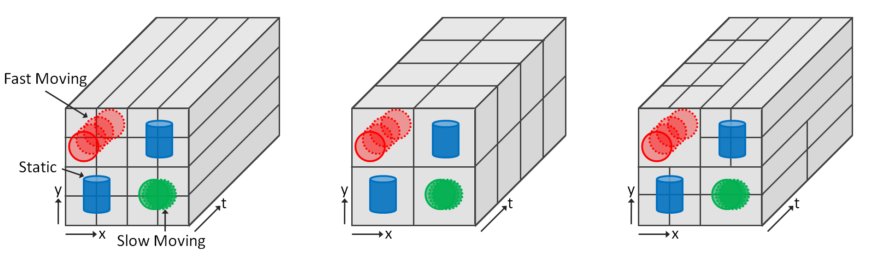
\includegraphics[width=8cm]{figures/flexible_voxels.png}};
%	\end{tikzpicture}
%	
%	\label{fig:flexible_voxels}
%	
%	\caption{Flexible voxels}
%\end{figure}

In \cite{Koller2015}, a prototype compressive video camera that encodes scene movement using a translated binary photo-mask in the optical path was presented. The encoded recording can be used to reconstruct multiple output frames from each captured image, effectively synthesizing high-speed video (see~Fig.~\ref{fig:temporal_cs}). Similarly, coded aperture compressive temporal imaging (CACTI) device proposed in \cite{Llull2013}, uses translating coded aperture during exposure to modulate each temporal plane in the video stream by a shifted version of the code, attaining per-pixel modulation using no additional sensor bandwidth. This process can be viewed as a form of code division multiple access (CDMA). The temporal channels are isolated from the compressed data by inverting a highly underdetermined system of equations and using an iterative reconstruction algorithm, several high-speed video frames are obtained from a single coded measurement. CACTI device was used in \cite{Llull2014} to estimate a sequence of video frames and to reconstruct an extended depth of field image from a single two-dimensional coded measurement.
%
\begin{figure}
	\centering
	\begin{tikzpicture}
	\node[anchor=center](rec1) at (0,0)
	{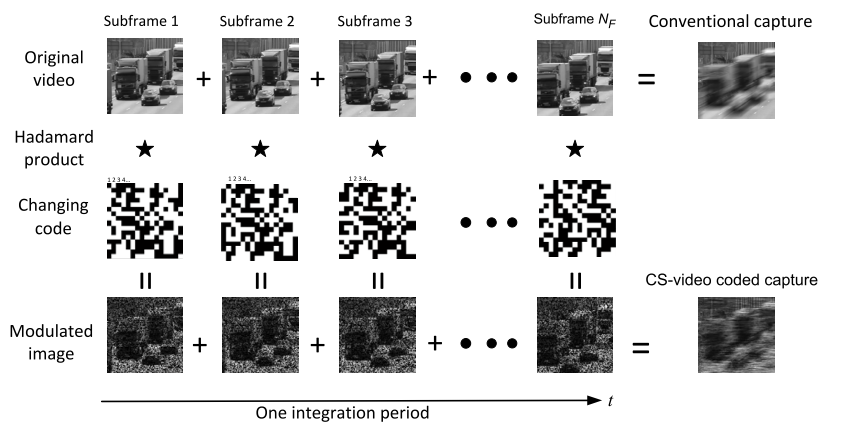
\includegraphics[width=8.6cm]{figures/temporal_cs.png}};
	\end{tikzpicture}
	
	\caption{Temporal compressive sensing model. A space-time volume $\boldsymbol{x}$ consisting of a set of $T$ frames, with $H\times W$ pixels each is multiplied by a set of mask patterns embedded within the sensing matrix $\boldsymbol{\Phi}$. The sensor integrates over time, producing a single coded captured image $\boldsymbol{y}$ consisting of $H\times W$ pixels. \cite{Koller2015}}
	
	\label{fig:temporal_cs}
\end{figure}


Light field imagers such as the plenoptic and integral imagers measure projections of 4D light field scalar function onto a two dimensional sensor and therefore suffer from a spatial vs. angular resolution trade-off. Several architectures for compressive light-field imaging that require relatively few photon-efficient measurements to obtain a high-resolution estimate of the light field have been proposed in \cite{Ashok2010, Babacan2012, Marwah2013}. These architectures offer a significant improvement over traditional light-field imagers exploiting spatio-angular correlations inherent in the light fields of natural scenes. The basic principle of utilizing a coded aperture to obtain light field images is depicted in Fig. \ref{fig:light_field_cs}.
%
\begin{figure}
	\centering
	\begin{tikzpicture}
	\node[anchor=center](rec1) at (0,0)
	{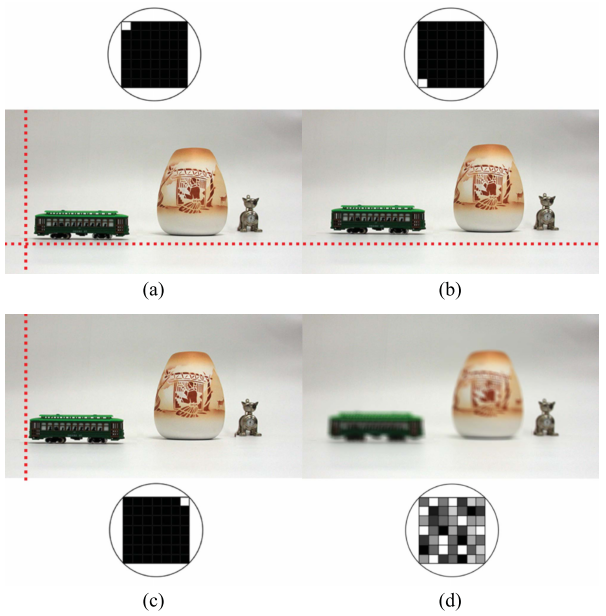
\includegraphics[width=8.6cm]{figures/light_field_cs.png}};
	\end{tikzpicture}
	
	\caption{Basic principle of utilizing a coded aperture to obtain light field images. (a)-(c) The angular images when only corner blocks of the aperture are left open. (d) Captured image with the randomly coded aperture used in the proposed compressive sensing light field camera. \cite{Babacan2012}}
	
	\label{fig:light_field_cs}
\end{figure}


Inspired by different compressive imaging architectures, we have designed a simple setup for compressive imaging consisting of off-the-shelf components. A simple and portable plug-and-play compressive imaging architecture consists of digital camera and projector. Our compressive imaging method allows the use of low-resolution camera even with strong lens distortion for measurement acquisition. Results of our compressive imaging method are non-distorted, high-resolution images which are obtained using compressive sensing reconstruction process on acquired measurement data (see Fig. \ref{fig:our_results}).
%
\begin{figure}
	\centering
	\begin{tikzpicture}
	\node[anchor=center](rec1) at (0,0)
	{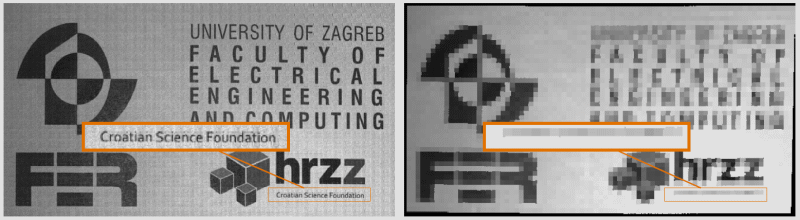
\includegraphics[width=8.6cm]{figures/cs_rec.png}};
	\end{tikzpicture}
	
	\caption{Reconstruction of a two-dimensional scene using compressive imaging system composed of a projector and a camera. Left image shows the scene reconstruction, while right image shows single measurement from the camera sensor.}
		
	\label{fig:our_results}
\end{figure}

%\hfill mds
 
%\hfill August 26, 2015

%\subsection{Subsection Heading Here}
%Subsection text here.

% needed in second column of first page if using \IEEEpubid
%\IEEEpubidadjcol

%\subsubsection{Subsubsection Heading Here}
%Subsubsection text here.


% An example of a floating figure using the graphicx package.
% Note that \label must occur AFTER (or within) \caption.
% For figures, \caption should occur after the \includegraphics.
% Note that IEEEtran v1.7 and later has special internal code that
% is designed to preserve the operation of \label within \caption
% even when the captionsoff option is in effect. However, because
% of issues like this, it may be the safest practice to put all your
% \label just after \caption rather than within \caption{}.
%
% Reminder: the "draftcls" or "draftclsnofoot", not "draft", class
% option should be used if it is desired that the figures are to be
% displayed while in draft mode.
%
%\begin{figure}[!t]
%\centering
%\includegraphics[width=2.5in]{myfigure}
% where an .eps filename suffix will be assumed under latex, 
% and a .pdf suffix will be assumed for pdflatex; or what has been declared
% via \DeclareGraphicsExtensions.
%\caption{Simulation results for the network.}
%\label{fig_sim}
%\end{figure}

% Note that the IEEE typically puts floats only at the top, even when this
% results in a large percentage of a column being occupied by floats.


% An example of a double column floating figure using two subfigures.
% (The subfig.sty package must be loaded for this to work.)
% The subfigure \label commands are set within each subfloat command,
% and the \label for the overall figure must come after \caption.
% \hfil is used as a separator to get equal spacing.
% Watch out that the combined width of all the subfigures on a 
% line do not exceed the text width or a line break will occur.
%
%\begin{figure*}[!t]
%\centering
%\subfloat[Case I]{\includegraphics[width=2.5in]{box}%
%\label{fig_first_case}}
%\hfil
%\subfloat[Case II]{\includegraphics[width=2.5in]{box}%
%\label{fig_second_case}}
%\caption{Simulation results for the network.}
%\label{fig_sim}
%\end{figure*}
%
% Note that often IEEE papers with subfigures do not employ subfigure
% captions (using the optional argument to \subfloat[]), but instead will
% reference/describe all of them (a), (b), etc., within the main caption.
% Be aware that for subfig.sty to generate the (a), (b), etc., subfigure
% labels, the optional argument to \subfloat must be present. If a
% subcaption is not desired, just leave its contents blank,
% e.g., \subfloat[].


% An example of a floating table. Note that, for IEEE style tables, the
% \caption command should come BEFORE the table and, given that table
% captions serve much like titles, are usually capitalized except for words
% such as a, an, and, as, at, but, by, for, in, nor, of, on, or, the, to
% and up, which are usually not capitalized unless they are the first or
% last word of the caption. Table text will default to \footnotesize as
% the IEEE normally uses this smaller font for tables.
% The \label must come after \caption as always.
%
%\begin{table}[!t]
%% increase table row spacing, adjust to taste
%\renewcommand{\arraystretch}{1.3}
% if using array.sty, it might be a good idea to tweak the value of
% \extrarowheight as needed to properly center the text within the cells
%\caption{An Example of a Table}
%\label{table_example}
%\centering
%% Some packages, such as MDW tools, offer better commands for making tables
%% than the plain LaTeX2e tabular which is used here.
%\begin{tabular}{|c||c|}
%\hline
%One & Two\\
%\hline
%Three & Four\\
%\hline
%\end{tabular}
%\end{table}


% Note that the IEEE does not put floats in the very first column
% - or typically anywhere on the first page for that matter. Also,
% in-text middle ("here") positioning is typically not used, but it
% is allowed and encouraged for Computer Society conferences (but
% not Computer Society journals). Most IEEE journals/conferences use
% top floats exclusively. 
% Note that, LaTeX2e, unlike IEEE journals/conferences, places
% footnotes above bottom floats. This can be corrected via the
% \fnbelowfloat command of the stfloats package.


%%%%%%%%%%%%%%%%%%%%%%%%%%%%%%%%%%%%%%%%%%%%%%%%%%%%%%%%%%%%%%%%%%%%%%%%%%%%%%%%%%%%%%%%%%%%%%%%%%%%%%%%%%%
%%%%%%%%%%%%%%%%%%%%%%%%%%%%%%%%%%%%%%%%%%%%%%%%%%%%%%%%%%%%%%%%%%%%%%%%%%%%%%%%%%%%%%%%%%%%%%%%%%%%%%%%%%%
\section{Conclusion} \label{sec:7}

In this paper, we gave an introduction to the theory of sparse signal modeling and compressive sensing. We covered basis representation fundamentals using an illustrative example, sparse signal recovery basics, desired properties of compressive sensing matrices and uniqueness of CS recovery problem. Furthermore, we provided overview of algorithms for sparse recovery and overcomplete dictionary learning. Finally, we showed numerous practical applications of compressive sensing framework on real-word problems. Compressive sensing offers novel signal acquisition and reconstruction framework. The traditional Shannon-Nyquist sampling theory in which successful recovery of a signal only depends on the bandwidth of the signal is replaced by novel compressive sensing framework where informational content of the signal dictates recovery success.

Compressive sensing has become an alternative for the well established Shannon-Nyquist sampling theory. However, there are several aspects of CS where further improvements are needed including sparse recovery algorithms, theoretical formulations and guarantees and finally, fundamental limits which will lead to novel and revolutionary practical applications solving real-world problems.




% if have a single appendix:
%\appendix[Proof of the Zonklar Equations]
% or
%\appendix  % for no appendix heading
% do not use \section anymore after \appendix, only \section*
% is possibly needed

% use appendices with more than one appendix
% then use \section to start each appendix
% you must declare a \section before using any
% \subsection or using \label (\appendices by itself
% starts a section numbered zero.)
%


%\appendices
%\section{Proof of the First Zonklar Equation}
%Appendix one text goes here.

% you can choose not to have a title for an appendix
% if you want by leaving the argument blank
%\section{}
%Appendix two text goes here.


% use section* for acknowledgment
%\section*{Acknowledgment}


%The authors would like to thank...


% Can use something like this to put references on a page
% by themselves when using endfloat and the captionsoff option.
\ifCLASSOPTIONcaptionsoff
  \newpage
\fi



% trigger a \newpage just before the given reference
% number - used to balance the columns on the last page
% adjust value as needed - may need to be readjusted if
% the document is modified later
%\IEEEtriggeratref{8}
% The "triggered" command can be changed if desired:
%\IEEEtriggercmd{\enlargethispage{-5in}}

% references section

% can use a bibliography generated by BibTeX as a .bbl file
% BibTeX documentation can be easily obtained at:
% http://mirror.ctan.org/biblio/bibtex/contrib/doc/
% The IEEEtran BibTeX style support page is at:
% http://www.michaelshell.org/tex/ieeetran/bibtex/
%\bibliographystyle{IEEEtran}
% argument is your BibTeX string definitions and bibliography database(s)
%\bibliography{IEEEabrv,../bib/paper}
%
% <OR> manually copy in the resultant .bbl file
% set second argument of \begin to the number of references
% (used to reserve space for the reference number labels box)



% biography section
% 
% If you have an EPS/PDF photo (graphicx package needed) extra braces are
% needed around the contents of the optional argument to biography to prevent
% the LaTeX parser from getting confused when it sees the complicated
% \includegraphics command within an optional argument. (You could create
% your own custom macro containing the \includegraphics command to make things
% simpler here.)
%\begin{IEEEbiography}[{\includegraphics[width=1in,height=1.25in,clip,keepaspectratio]{mshell}}]{Michael Shell}
% or if you just want to reserve a space for a photo:

%\begin{IEEEbiography}{Michael Shell}
%Biography text here.
%\end{IEEEbiography}
%%%%%%%%%%%%%%%%%%%%%%%%%%%%%%%%%%%%%%%%%%%%%%%%%%%%%%%%%%%%%%%%%%%%%%%%%%%%%%%%%%%%%%%%%%%%%%%%%%%%%%%%%%%
%%%%%%%%%%%%%%%%%%%%%%%%%%%%%%%%%%%%%%%%%%%%%%%%%%%%%%%%%%%%%%%%%%%%%%%%%%%%%%%%%%%%%%%%%%%%%%%%%%%%%%%%%%%
\bibliographystyle{IEEEtran}
\bibliography{IEEEabrv,references}


% You can push biographies down or up by placing
% a \vfill before or after them. The appropriate
% use of \vfill depends on what kind of text is
% on the last page and whether or not the columns
% are being equalized.

%\vfill

% Can be used to pull up biographies so that the bottom of the last one
% is flush with the other column.
%\enlargethispage{-5in}



% that's all folks
\end{document}


